\documentclass[11pt,oneside]{book}

\title{OpenUSD Exam Companion}
\newcommand{\booksubtitle}{NCP-OUSD Prep Notes and Tested Examples}
% \newcommand{\booktagline}{Cheat sheets, drills, tested examples, and original practice questions}
\newcommand{\booklicense}{Creative Commons Attribution--NonCommercial--NoDerivatives 4.0 International (CC BY-NC-ND 4.0)}
\author{David Khosid}
\newcommand{\edition}{v0.02 Edition}

\makeatletter
\newcommand{\booktitle}{\@title}
\newcommand{\bookauthor}{\@author}
\makeatother

\usepackage[utf8]{inputenc}
\usepackage{fix-cm}
\usepackage{lmodern}
\usepackage{tikz}
\usepackage{amsmath}
\usepackage{amssymb}
\usepackage{microtype}
\usepackage{graphicx}
\usepackage{hyperref}
\usepackage{bookmark}
\usepackage{enumitem}
\usepackage{fancyhdr}
\usepackage{xcolor}
\usepackage{makeidx}
\makeindex

\usepackage[bindingoffset=0.625in,
            left=.5in, right=.5in,
            top=.8125in, bottom=.9375in,
            marginparwidth=27pt, marginparsep=5pt,
            paperwidth=6.375in, paperheight=9.25in]{geometry}
\usepackage{marginnote}

\hypersetup{
  colorlinks=true,
  linkcolor=blue,
  urlcolor=blue,
  citecolor=blue,
  pdftitle={OpenUSD Exam Companion},
  pdfauthor={David Khosid}
}

\pagestyle{fancy}
\fancyhf{}
\fancyhead[LE,RO]{\thepage}
\fancyhead[LO]{\nouppercase{\rightmark}}
\fancyhead[RE]{\nouppercase{\leftmark}}
\renewcommand{\headrulewidth}{0.4pt}

\setlist[itemize]{itemsep=2pt, topsep=3pt}

% Avoid fancyhdr headheight warnings
\setlength{\headheight}{14pt}

\usepackage{listings}

% Listing palette (print-safe: keywords stay bold for grayscale printing)
\definecolor{usdKeyword}{HTML}{0550AE}   % structural keywords / metadata keys
\definecolor{usdType}{HTML}{8250DF}      % value types
\definecolor{usdString}{HTML}{0A7B30}    % strings
\definecolor{usdComment}{HTML}{6E7781}   % comments and the #usda cookie
\definecolor{usdNew}{HTML}{B45309}       % lines just authored (produces idiom)
\definecolor{usdFrame}{HTML}{C4C9CE}
\definecolor{usdBg}{HTML}{FAFAF7}

\lstdefinelanguage{USDA}{
  morekeywords={def,over,class,variantSet,variants,variantSets,
    prepend,append,add,delete,reorder,
    references,payload,inherits,specializes,subLayers,
    uniform,custom,rel,
    defaultPrim,upAxis,metersPerUnit,startTimeCode,endTimeCode,
    kind,apiSchemas,instanceable,active,bindMaterialAs,
    offset,scale,timeSamples},
  morekeywords=[2]{token,string,asset,bool,int,float,double,
    double3,float3,int2,color3f,point3f,normal3f,vector3d,
    matrix4d,texCoord2f,quatf},
  sensitive=true,
  morecomment=[l]{\#},
  morestring=[b]",
}

% Keep each example on one page: box every listing whole. A listing taller
% than the text column must opt out with \AllowListingBreak on the line
% before it (the flag resets after one use).
\usepackage{etoolbox}
\newif\ifLongListing
\newcommand{\AllowListingBreak}{\global\LongListingtrue}
\BeforeBeginEnvironment{lstlisting}{%
  \ifLongListing\else\par\vspace{0pt minus 3pt}\noindent
  \begin{minipage}{\linewidth}\fi}
\AfterEndEnvironment{lstlisting}{%
  \ifLongListing\global\LongListingfalse\else\end{minipage}\par\fi}

\lstset{
  language=USDA,
  basicstyle=\ttfamily\small,
  keywordstyle=\bfseries\color{usdKeyword},
  keywordstyle=[2]\color{usdType},
  stringstyle=\color{usdString},
  commentstyle=\itshape\color{usdComment},
  columns=fullflexible,
  frame=single,
  rulecolor=\color{usdFrame},
  backgroundcolor=\color{usdBg},
  breaklines=true,
  tabsize=2,
  showstringspaces=false,
  aboveskip=0.55em,
  belowskip=0.45em,
  % "produces" idiom: a line starting with ";;" renders without the marker,
  % bold and amber — marking scene description that the code just authored.
  moredelim=**[il][\bfseries\color{usdNew}]{;;},
}

% Shared visual language for composition / scenegraph diagrams.
% Every figure in the book uses these styles: one palette, one look.
\usetikzlibrary{arrows.meta,positioning,calc}

% Palette
\definecolor{usdgreen}{HTML}{76B900}   % accent green
\definecolor{arcRef}{HTML}{1F6FEB}     % references
\definecolor{arcPay}{HTML}{D9730D}     % payloads
\definecolor{arcVar}{HTML}{0E8A8A}     % variant sets
\definecolor{arcInh}{HTML}{7C3AED}     % inherits
\definecolor{arcSpec}{HTML}{57606A}    % specializes
\definecolor{layerFill}{HTML}{F3F8E8}  % layer boxes
\definecolor{primFill}{HTML}{F6F8FA}   % prim boxes

\tikzset{
  layerbox/.style={draw=usdgreen!60!black, fill=layerFill, rounded corners=2pt,
    minimum width=3.0cm, minimum height=0.66cm, font=\small\ttfamily},
  primbox/.style={draw=black!55, fill=primFill, rounded corners=2pt,
    minimum width=2.4cm, minimum height=0.6cm, font=\small\ttfamily},
  strengthbox/.style={draw=black!50, fill=black!4, rounded corners=2pt,
    text width=8.6cm, minimum height=0.62cm, align=left,
    font=\small\sffamily},
  notetext/.style={font=\scriptsize\sffamily, text=black!70},
  arc/.style={-{Stealth[length=2.6mm]}, thick},
  refArc/.style={arc, draw=arcRef},
  payArc/.style={arc, draw=arcPay, dashed},
  varArc/.style={arc, draw=arcVar},
  inhArc/.style={arc, draw=arcInh, densely dotted},
  specArc/.style={arc, draw=arcSpec, densely dotted},
  subArc/.style={arc, draw=usdgreen!60!black},
  arcLabel/.style={font=\scriptsize\sffamily, midway, sloped, above},
}

% Callout boxes. Uses the palette from styles/diagrams.tex.
\usepackage[most]{tcolorbox}

\newtcolorbox{ExamTip}{enhanced,
  colback=usdgreen!7, colframe=usdgreen!60!black,
  title=Exam Tip, fonttitle=\bfseries\sffamily\small,
  boxrule=0.6pt, arc=1.5pt,
  left=4pt, right=4pt, top=3pt, bottom=3pt,
  before skip=0.9em, after skip=0.9em}

\newtcolorbox{Gotcha}{enhanced,
  colback=arcPay!8, colframe=arcPay!85!black,
  title=Gotcha, fonttitle=\bfseries\sffamily\small,
  boxrule=0.6pt, arc=1.5pt,
  left=4pt, right=4pt, top=3pt, bottom=3pt,
  before skip=0.9em, after skip=0.9em}

\newtcolorbox{DeepDive}{enhanced,
  colback=arcRef!6, colframe=arcRef!70!black,
  title=Deep Dive, fonttitle=\bfseries\sffamily\small,
  boxrule=0.6pt, arc=1.5pt,
  left=4pt, right=4pt, top=3pt, bottom=3pt,
  before skip=0.9em, after skip=0.9em}

\newtcolorbox{FieldNote}{enhanced,
  colback=arcInh!6, colframe=arcInh!70!black,
  title=Field Note, fonttitle=\bfseries\sffamily\small,
  boxrule=0.6pt, arc=1.5pt,
  left=4pt, right=4pt, top=3pt, bottom=3pt,
  before skip=0.9em, after skip=0.9em}

\newtcolorbox{DrillSolution}{enhanced,
  colback=black!4, colframe=black!40,
  title=Solution, fonttitle=\bfseries\sffamily\small,
  boxrule=0.5pt, arc=1.5pt,
  left=4pt, right=4pt, top=3pt, bottom=3pt,
  before skip=0.6em, after skip=0.9em}

\newcommand{\DomainHeader}[2]{
  \chapter{#1}
  \noindent\textbf{Exam Weight:} #2\par\vspace{0.4em}
}

\newenvironment{Objectives}{\section{Objectives}\begin{itemize}[leftmargin=*]}{\end{itemize}}
\newenvironment{Resources}{\section{Recommended resources}\begin{itemize}[leftmargin=*]}{\end{itemize}}

% Margin tag tying a passage to numbered study-guide objectives, e.g.
% \objref{1.6} or \objref{1.10, 2.5}. Bare numbers; domain prefixes implied
% by the guide's numbering (1=Composition ... 8=Visualization).
% Each number is a link to its row in the Coverage Map (\objrow anchors).
\makeatletter
\newcommand{\obj@strip}[1]{\edef\obj@n{\zap@space#1 \@empty}}
\newcommand{\objref}[1]{\marginnote{%
  \raggedright\scriptsize\sffamily
  \def\obj@sep{}%
  \@for\obj@n:=#1\do{%
    \expandafter\obj@strip\expandafter{\obj@n}%
    \obj@sep\hyperlink{obj:\obj@n}{\textcolor{black!55}{\obj@n}}%
    \def\obj@sep{, }}%
}}
\makeatother
% Coverage-map row anchor: prints the objective number and registers the
% jump target for \objref, raised a line so the row lands below the jump.
\newcommand{\objrow}[1]{%
  \raisebox{1.2\baselineskip}[0pt][0pt]{\hypertarget{obj:#1}{}}#1}

% Connector for the "code -> produces -> scene description" idiom (adopted
% from the official OpenUSD tutorials). Mark authored lines in the second
% listing by starting them with ";;".
\newcommand{\produces}{\par\nopagebreak\noindent\textit{\small produces}\par\nopagebreak\vspace{0.1em}}

% Compact question header for the practice chapters (replaces the roomy
% starred subsections) and a bullet-free, tight answer-choice list — the
% A./B./C. labels make bullets redundant.
\newcommand{\Question}[1]{\par\vspace{0.9em plus 0.3em}%
  \noindent\textbf{Question #1}\par\nopagebreak\vspace{0.2em}\ignorespaces}
\newenvironment{Choices}
  {\begin{itemize}[leftmargin=1.5em, label={}, itemsep=1pt, topsep=2pt,
    parsep=0pt]}
  {\end{itemize}}

\newcommand{\CheatSheetTitle}{\section*{Cheat Sheet (one page)}\addcontentsline{toc}{section}{Cheat Sheet}}
\newcommand{\DrillsTitle}{\section*{Exercises and Drills}\addcontentsline{toc}{section}{Exercises and Drills}}

\newcommand{\AnswerLines}[1]{%
  \par\nopagebreak\vspace{0.2em}\nopagebreak\noindent
  \rule{\textwidth}{0.4pt}\par
  \vspace{0.2em}
  \noindent\textit{Write here:}\par
  \vspace{0.2em}
  \foreach \i in {1,...,#1}{\noindent\rule{\textwidth}{0.4pt}\par\vspace{0.55em}}%
}

\newcommand{\HalfTitlePage}{
  \newgeometry{top=1.75in,bottom=.5in}
  \begin{titlepage}
  \begin{flushleft}
  \textbf{\fontfamily{qcs}\fontsize{44}{50}\selectfont OpenUSD\\Exam\\Companion\\}
  \par\noindent\rule{\textwidth}{4pt}\\[6pt]
  
\begin{tikzpicture}
  \shade[bottom color=usdgreen!22,top color=white]
      (0,0) rectangle (\textwidth, 1.6)
      node[midway] {\parbox{0.92\textwidth}{\centering\textbf{\large \textit{\booksubtitle}}}};
  \end{tikzpicture}
  \begin{flushright}\Large \edition\end{flushright}
  \vspace{\fill}
  \end{flushleft}
  \end{titlepage}
  \restoregeometry
}

\newcommand{\TitlePage}{
  \thispagestyle{empty}
  \newgeometry{top=1.75in,bottom=.5in}
  \begin{titlepage}
  \begin{flushleft}
  \textbf{\fontfamily{qcs}\fontsize{44}{50}\selectfont \booktitle\\}
  \par\noindent\rule{\textwidth}{4pt}\\[6pt]
  
\begin{tikzpicture}
  \shade[bottom color=usdgreen!22,top color=white]
      (0,0) rectangle (\textwidth, 1.6)
      node[midway] {\parbox{0.92\textwidth}{\centering\textbf{\large \textit{\booksubtitle}}}};
  \end{tikzpicture}
  \begin{flushright}\Large \edition\end{flushright}
  \vspace{\fill}
  \textbf{\large \bookauthor}
  \vspace{\fill}
  \end{flushleft}
  \end{titlepage}
  \restoregeometry
}

\newcommand{\ColophonPage}{
  \thispagestyle{empty}
  \begin{flushleft}
  \vspace*{\fill}
  This book was typeset using \LaTeX{}. Every USD example in it was executed
  against a real OpenUSD build before publication.\\[1.2em]
  This is an independent publication. It is not affiliated with, endorsed by,
  or sponsored by NVIDIA Corporation. NVIDIA and NCP-OUSD are trademarks of
  NVIDIA Corporation, used here for identification purposes only.\\
  \vspace{\fill}
  Copyright \textcopyright{} \the\year{} \bookauthor\\[0.6em]
  Licensed under the \booklicense.\\
  You may share verbatim copies of this book freely for non-commercial
  purposes, with attribution. Commercial distribution and derivative works
  require the author's permission.\\
  \url{https://creativecommons.org/licenses/by-nc-nd/4.0/}
  \end{flushleft}
}


\begin{document}
\frontmatter
\HalfTitlePage
\TitlePage
\ColophonPage

\chapter*{Preface}
\addcontentsline{toc}{chapter}{Preface}
This companion is structured around NVIDIA’s \textit{NCP: OpenUSD Development Exam Study Guide (v1.1.0)}.
It reorganizes the blueprint into a book-like flow and adds space for notes, drills, and checklists.

\bigskip
\noindent\textbf{How to use this book}
\begin{itemize}[leftmargin=*]
  \item For each domain: read the cheat sheet, work the drills, then do the questions.
  \item Work each drill before reading the solution beneath it --- on paper if
        you printed the book, out loud or in your notes if you are reading the
        PDF. The recall attempt is the exercise; the solution is the check.
  \item Keep a running “gotchas” list (composition strength, instancing edits, material binding, etc.).
  \item Revisit the sample questions after each domain.
\end{itemize}

\setcounter{tocdepth}{2}
\tableofcontents

\mainmatter
\input{chapters/00-intro}
\chapter{Exam Blueprint}
\section{Domains and Weights}
\begin{itemize}[leftmargin=*]
  \item Composition — 23\%
  \item Content Aggregation — 10\%
  \item Customizing USD — 6\%
  \item Data Exchange — 15\%
  \item Data Modeling — 13\%
  \item Debugging and Troubleshooting — 11\%
  \item Pipeline Development — 14\%
  \item Visualization — 8\%
\end{itemize}

\section{How to study (fast feedback loop)}
\begin{itemize}[leftmargin=*]
  \item Read cheat sheet $\rightarrow$ do drills $\rightarrow$ explain to yourself $\rightarrow$ re-run drills.
  \item Prefer tiny USD layers you can reason about (3–20 lines).
  \item Always ask: “Which layer wins and why?” (LIVRPS + strength).
\end{itemize}

\section{Field notes from test-takers}
Synthesized from public write-ups by certified developers and from this
author's own attempts --- the things people consistently wish they had known
before booking the exam.

\begin{itemize}[leftmargin=*]
  \item \textbf{Experience does not equal readiness.} Developers with years
        of production USD and Omniverse work report failing a first attempt
        after $\sim$80 hours of study. The exam tests the guide's objectives
        \emph{specifically} --- including domains your daily work never
        touches.
  \item \textbf{Budget 80--120 focused hours} over 8--10 weeks. People who
        passed recommend at least 100; under-investment is the most-cited
        cause of first-attempt failures.
  \item \textbf{Work the guide point by point.} Coverage beats extra depth in
        your comfort zone. The margin tags and the Coverage Map appendix in
        this book exist for exactly that: no objective left unvisited.
  \item \textbf{Composition dominates --- mentally.} Expect LIVRPS scenarios
        you must trace \emph{without} usdview. Practice predicting the
        composed result first and verifying second; then practice with the
        verification switched off.
  \item \textbf{It is a Python exam.} API questions use the Python surface;
        read and write \texttt{pxr} code fluently.
  \item \textbf{Understand the wrong answers.} For every practice question,
        articulate why each distractor fails --- this book's answer key is
        written that way on purpose. Then build your own variant of the
        scenario; the drills exist for exactly this.
\end{itemize}

\noindent\textbf{Logistics.} The exam is remotely proctored (Certiverse),
costs about \$200, and the certification is valid for two years. A failed
attempt can be retaken after 14 days, up to five attempts per year --- plan
your calendar so a retake is an option, not a crisis. For hands-on practice,
\texttt{usdview} alone is sufficient tooling; no special hardware is needed.


\part{Domains}
\input{chapters/10-composition}
\input{chapters/11-content-aggregation}
\DomainHeader{Customizing USD}{6\%}

\begin{Objectives}
  \item Build a USD plug-in against a specific USD version.
  \item Build USD from source with custom dependencies.
  \item Create custom model kinds when appropriate.
  \item Create custom schemas for proprietary data models.
  \item Integrate a custom resolver for dynamic asset paths.
  \item Use schemas for nonstandard attributes/structures during import/export.
  \item Write a SceneIndex plug-in that generates Hydra prims.
  \item Write an AssetResolver that generates in-memory renderable primitives.
\end{Objectives}

\begin{Resources}
  \item Learn OpenUSD: Understanding Model Kinds
  \item OpenUSD tutorial: Generating New Schema Classes (usdGenSchema)
  \item Whitepaper: What Are OpenUSD Schemas?
  \item OpenUSD API: PlugRegistry; Kind --- Extensible Categorization;
        Ar (Asset Resolution); file format plug-ins
\end{Resources}

\CheatSheetTitle
\begin{itemize}[leftmargin=*]
  \item \textbf{Everything pluggable goes through one door}:
        \texttt{plugInfo.json} files on \texttt{PXR\_PLUGINPATH\_NAME},
        loaded by \texttt{PlugRegistry} --- schemas, kinds, file formats,
        resolvers, Hydra plug-ins.\index{plugInfo.json}\index{PlugRegistry}
  \item \textbf{Typed (IsA) schema}: defines a new prim type
        (\texttt{def SimJoint}). \textbf{API schema}: adds properties and
        behavior to \emph{existing} types (applied; recorded in
        \texttt{apiSchemas} metadata).\index{IsA schema}\index{API schema}
  \item \textbf{usdGenSchema} turns a \texttt{schema.usda} description into
        registered schemas; with \texttt{skipCodeGeneration = true} they are
        \emph{codeless} --- deployable without compiling.\index{usdGenSchema}\index{codeless schema}
  \item \textbf{The formality ladder}: ad-hoc custom attributes $\to$
        namespaced conventions $\to$ API schema $\to$ typed schema. Climb
        only when querying/validation/tooling demands it.
  \item \textbf{Custom kinds} extend the model hierarchy vocabulary via
        plugInfo (\texttt{"vehicle" baseKind "component"}) --- every site
        that opens your assets needs the same registration.\index{kind}
  \item \textbf{Ar resolver}: logical identifier $\to$ resolved path;
        contexts pin versions/sites. \textbf{File format plug-in}: teaches
        USD to read a foreign format \emph{as} scene description.
        \textbf{SceneIndex}: procedurally feeds Hydra prims at render time.
  \item \textbf{Version pinning}: plug-ins link against one exact USD
        build --- ABI compatibility is per-version, so match headers,
        compiler, and flags.
\end{itemize}

\section{Core Concepts}

\subsection{The plugin map}\label{sec:cu-map}\objref{3.1}

\begin{figure}[ht]
  \centering
  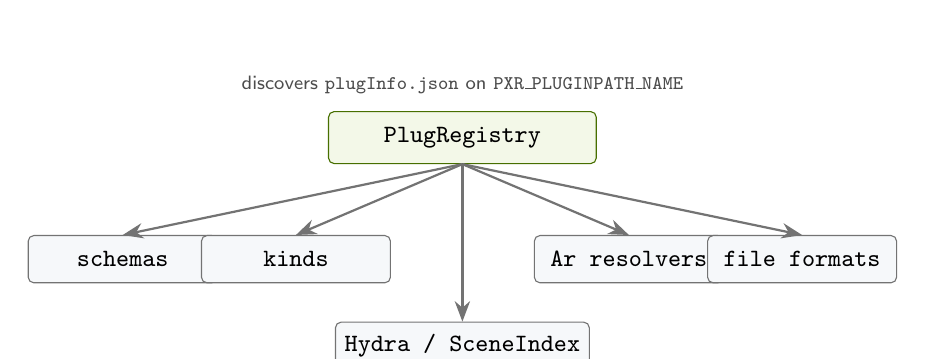
\begin{tikzpicture}[node distance=5mm and 8mm]
    \node[layerbox, minimum width=3.4cm] (reg) {PlugRegistry};
    \node[notetext, above=1mm of reg] {discovers \texttt{plugInfo.json} on \texttt{PXR\_PLUGINPATH\_NAME}};
    \node[primbox, below left=9mm and 14mm of reg] (schemas) {schemas};
    \node[primbox, below left=9mm and -8mm of reg] (kinds) {kinds};
    \node[primbox, below right=9mm and -8mm of reg] (ar) {Ar resolvers};
    \node[primbox, below right=9mm and 14mm of reg] (ff) {file formats};
    \node[primbox, below=20mm of reg] (hydra) {Hydra / SceneIndex};
    \draw[arc, draw=black!55] (reg.south) -- (schemas.north);
    \draw[arc, draw=black!55] (reg.south) -- (kinds.north);
    \draw[arc, draw=black!55] (reg.south) -- (ar.north);
    \draw[arc, draw=black!55] (reg.south) -- (ff.north);
    \draw[arc, draw=black!55] (reg.south) -- (hydra.north);
  \end{tikzpicture}
  \caption{One discovery mechanism, five common extension points. If a
  plug-in ``doesn't load'', debug the door first:
  \texttt{TF\_DEBUG=PLUG\_REGISTRATION}.}
  \label{fig:plugin-map}
\end{figure}

\subsection{Custom schemas: describe once, generate the rest}\label{sec:cu-schemas}\objref{3.4, 3.6}
\index{usdGenSchema}A proprietary data model becomes a first-class USD
citizen through a \texttt{schema.usda} description that
\texttt{usdGenSchema} consumes:

\begin{lstlisting}
#usda 1.0
(
    subLayers = [@usd/schema.usda@]
)
over "GLOBAL" (
    customData = {
        string libraryName = "simRobot"
        string libraryPath = "."
        bool skipCodeGeneration = true
    }
)
{
}
class SimJoint "SimJoint" (
    inherits = </Typed>
)
{
    float torqueLimit = 100 (
        doc = "Maximum torque in Nm."
    )
}
class "WearAPI" (
    inherits = </APISchemaBase>
    customData = {
        token apiSchemaType = "singleApply"
    }
)
{
    float wearAmount = 0 (
        doc = "0 = pristine, 1 = destroyed."
    )
}
\end{lstlisting}

\noindent One file declares both flavors: \texttt{SimJoint} is a
\emph{typed} (IsA) schema --- prims can be \texttt{def SimJoint} --- and
\texttt{WearAPI} is an \emph{applied API} schema that any existing prim type
can opt into. With \texttt{skipCodeGeneration = true} the result is a
\emph{codeless} schema: registered purely as data (plugInfo +
generated schema layer), no C++ to compile or deploy --- the modern default
for pipeline schemas.\index{codeless schema}

\begin{ExamTip}
Typed vs API in one breath: \emph{is it a thing, or a capability of existing
things?} New prim type with its own identity $\Rightarrow$ typed/IsA.
Extra properties for prims that already have a type (physics on meshes,
wear on props) $\Rightarrow$ applied API schema. Reach for schemas at all
only when ad-hoc namespaced attributes stop being enough --- fallbacks,
docs, validation, generated accessors.
\end{ExamTip}

\subsection{Applied API schemas in action}\label{sec:cu-api}\objref{3.4}
Application is recorded on the prim (in \texttt{apiSchemas} metadata) and
queryable --- here with a built-in multiple-apply schema, which behaves
exactly like the ones usdGenSchema generates for you:

\begin{lstlisting}[language=Python]
from pxr import Usd, UsdGeom

stage = Usd.Stage.CreateInMemory()
prim = UsdGeom.Xform.Define(stage, "/Robot").GetPrim()

Usd.CollectionAPI.Apply(prim, "render")
print(prim.HasAPI(Usd.CollectionAPI))   # True
print(prim.GetAppliedSchemas())         # ['CollectionAPI:render']
\end{lstlisting}

\noindent\texttt{Apply()} records the intent, \texttt{HasAPI()} answers
cheaply, and multiple-apply schemas take an instance name (here
\texttt{render}) so one capability can exist several times on a prim.

\subsection{Building USD itself}\label{sec:cu-build}\objref{3.2, 3.1}
\index{build\_usd.py}Sometimes the pipeline needs its own USD: a DCC ships
one build, the farm needs another, or a plug-in requires components the
prebuilt binaries exclude. The supported path is the repository's
\texttt{build\_usd.py}, which fetches dependencies and drives CMake; the
decisions that matter are the flags --- \texttt{--no-imaging} (core only, no
Hydra) for headless services, \texttt{--no-python} for embedded use,
optional components like MaterialX or OpenVDB, and monolithic vs shared
libraries. ``Custom dependencies'' in practice means pinning versions ---
TBB, MaterialX, OpenSubdiv, and above all the \emph{compiler and flags},
because every plug-in must be built with the same toolchain as the USD that
loads it.

\begin{ExamTip}
Exam framing for ``build USD from source'': component control (strip
imaging on a farm), dependency pinning to match a DCC's runtime, and ABI
parity for in-house plug-ins. Know the tool's name ---
\texttt{build\_usd.py} --- and that prebuilt binaries (pip
\texttt{usd-core}, NVIDIA releases) trade those choices away for
convenience.
\end{ExamTip}

\subsection{Custom kinds}\label{sec:cu-kinds}\objref{3.3}
\index{kind}The kind vocabulary itself is extensible --- a
\texttt{plugInfo.json} resource registers new kinds into the hierarchy:

\begin{lstlisting}
{
    "Plugins": [{
        "Type": "resource",
        "Name": "studioKinds",
        "Info": {
            "Kinds": {
                "vehicle": { "baseKind": "component" }
            }
        }
    }]
}
\end{lstlisting}

\noindent\texttt{baseKind} slots the new kind into existing semantics ---
a \texttt{vehicle} \emph{is a} component, so model-hierarchy tools keep
working. Create custom kinds when tools must select your category
(``all vehicles''), and remember the registration must exist on
\emph{every} site that consumes the assets --- kinds are vocabulary, not
data.

Registration end to end is exactly two steps: put the
\texttt{plugInfo.json} in a directory, put that directory on
\texttt{PXR\_PLUGINPATH\_NAME}. Verification is three lines --- and this
book's test suite runs precisely this in a subprocess against the
\texttt{plugInfo.json} printed above:

\begin{lstlisting}[language=Python]
# PXR_PLUGINPATH_NAME=/studio/plugins/studio_kinds python
from pxr import Kind

print(Kind.Registry.HasKind("vehicle"))      # True
print(Kind.Registry.GetBaseKind("vehicle"))  # component
\end{lstlisting}

\noindent Codeless schemas ride the same mechanism --- their plugin
directory carries a \texttt{generatedSchema.usda} plus a
\texttt{plugInfo.json} with \texttt{Types} entries. Let
\texttt{usdGenSchema} generate both from your \texttt{schema.usda}:
the \texttt{Types} block encodes TfType registration details that are
easy to get subtly wrong by hand.

\subsection{Resolvers, file formats, and SceneIndex --- who does what}\label{sec:cu-ext}\objref{3.5, 3.7, 3.8}
Three extension points get conflated on exams; the boundaries are clean:

An \textbf{Ar resolver}\index{resolver} answers ``\emph{where} is asset
\texttt{X}?'' --- it maps logical identifiers
(\texttt{asset://props/chair?version=latest}) to concrete resolved paths,
honoring contexts (site, show, pin file). It never parses content.

A \textbf{file format plug-in}\index{file format plug-in} answers ``how do I
read \emph{this kind of file} as USD?'' --- it parses a foreign format into
scene description on demand (that is how \texttt{usda}/\texttt{usdc}/Alembic
themselves are wired in). Dynamic file formats can even \emph{generate}
prims from parameters.

A \textbf{SceneIndex plug-in}\index{SceneIndex} sits on the Hydra side:
it filters or procedurally generates \emph{render} prims after composition
--- geometry the stage never authored (the ``in-memory renderable
primitives'' objective lives here and in dynamic file formats).

\begin{Gotcha}
``Build a plug-in against a specific USD version'' is not ceremony: USD's
C++ ABI changes between releases, so a plug-in must be compiled against the
\emph{exact} USD build that loads it --- same version, same compiler
family, same flags. A plug-in built for a studio's USD 24.08 will not load
into the pip \texttt{usd-core} of a different version; the symptom is a
silent non-load, and the diagnosis is \texttt{TF\_DEBUG=PLUG\_REGISTRATION}.
\end{Gotcha}

\DrillsTitle
\subsection*{Drill 1: Typed vs API schema}
Give 2 examples of when you would choose each.
\AnswerLines{6}
\begin{DrillSolution}
Typed/IsA: a robot joint (\texttt{SimJoint}) or a studio-specific camera rig
--- entities with their own identity that prims \emph{are}. Applied API:
physics properties on existing meshes, wear/aging data on any prop ---
capabilities added to prims that already have a type. Heuristic: \emph{is}
vs \emph{has}.
\end{DrillSolution}

\subsection*{Drill 2: Resolver design}
Sketch an example: \texttt{asset://chair?variant=oak} $\rightarrow$ actual
file path.
\AnswerLines{7}
\begin{DrillSolution}
The resolver parses scheme + identifier + query; consults its context (show
config, pin file) for the published version; returns e.g.\
\texttt{/site/assets/chair/v012/chair\_oak.usdc}. Scene files keep the
logical URI; re-pinning the context retargets every scene at once. Cache
invalidation and farm/workstation context parity are the two operational
risks.
\end{DrillSolution}

\subsection*{Drill 3: Pick the mechanism}
Custom attribute, API schema, typed schema, or custom kind --- one per case:
(a) per-prim review notes; (b) ``all vehicles'' selection in tools; (c) a
new \texttt{ConveyorBelt} entity; (d) torque limits on existing joints
across shows.
\AnswerLines{6}
\begin{DrillSolution}
(a) namespaced custom attribute (or \texttt{customData} if untyped and
unsampled); (b) custom kind with \texttt{baseKind = component}; (c) typed
schema; (d) applied API schema --- shared, documented, validatable across
shows.
\end{DrillSolution}

\section*{Checkpoint Questions}
\addcontentsline{toc}{section}{Checkpoint Questions}

\noindent\textbf{CQ1.} A colleague's new schema ``does nothing'' on the farm
but works locally. First two checks?
\begin{DrillSolution}
Is the plugin discoverable there (\texttt{PXR\_PLUGINPATH\_NAME} includes
its \texttt{plugInfo.json}? \texttt{TF\_DEBUG=PLUG\_REGISTRATION}), and is
the farm's USD the same version/ABI the plug-in was built against? Codeless
schemas dodge the second problem entirely.
\end{DrillSolution}

\noindent\textbf{CQ2.} Why are codeless schemas the default recommendation
for pipeline data models?
\begin{DrillSolution}
They deploy as data: no compilation, no ABI coupling, no per-platform
builds --- just plugInfo + the generated schema layer on the plugin path.
You give up generated C++/Python accessor classes; generic
\texttt{UsdPrim}/\texttt{UsdAttribute} access and \texttt{HasAPI} still
work.
\end{DrillSolution}

\noindent\textbf{CQ3.} Match the objective to the extension point:
``generate renderable prims that were never authored on the stage.''
\begin{DrillSolution}
Hydra-side generation --- a SceneIndex plug-in (or, upstream of render, a
dynamic file format producing prims from parameters). An Ar resolver is the
wrong answer by definition: it locates content, it does not create it.
\end{DrillSolution}

\subsection*{Mini-checklist (tick when mastered)}
\begin{itemize}[leftmargin=*]
  \item[$\square$] I can explain what a resolver does in one sentence.
  \item[$\square$] I can justify a schema over ad-hoc attrs --- and codeless over compiled.
  \item[$\square$] I can place kinds/schemas/formats/resolvers/SceneIndex on the plugin map.
  \item[$\square$] I know why plug-ins pin exact USD versions.
\end{itemize}

\input{chapters/13-data-exchange}
\DomainHeader{Data Modeling}{13\%}

\begin{Objectives}
  \item Add a primvar to a mesh.
  \item Choose correct value types for attribute data.
  \item Represent custom metadata.
  \item Retrieve properties of a prim.
  \item Diagnose causes of unexpected visual results.
  \item Update \texttt{extent} after updating \texttt{points}.
\end{Objectives}

\begin{Resources}
  \item Learn OpenUSD: Setting the Stage; Scene Description Blueprints; Beyond
        the Basics
  \item User guide: Rendering --- Working With Primvars
  \item OpenUSD glossary: TimeCode; Layer Offset; List Editing; Primvar
  \item OpenUSD API: Sdf datatypes; UsdGeomPrimvar; Boundable; XformCache;
        UsdAttribute interpolation
\end{Resources}

\CheatSheetTitle
\begin{itemize}[leftmargin=*]
  \item \textbf{Two property kinds}: \emph{attributes} carry typed values
        (defaults + time samples); \emph{relationships} carry targets (paths).
        \index{attribute}\index{relationship}
  \item \textbf{Metadata is not an attribute}: it hangs on prims, properties,
        layers, or the stage; it is \emph{never} time-sampled
        (\texttt{kind}, \texttt{assetInfo}, \texttt{customData}).\index{metadata}
  \item \textbf{Primvars} are namespaced attributes (\texttt{primvars:*}) with
        an \emph{interpolation}: constant, uniform (per face), vertex,
        faceVarying --- and optional \texttt{:indices}.\index{primvar}
  \item \textbf{Value types carry meaning}: \texttt{color3f} vs
        \texttt{point3f} vs \texttt{normal3f} vs \texttt{vector3f} are all
        three floats --- the \emph{role} drives transformation and color
        handling.
  \item \textbf{token} for closed vocabularies, \texttt{string} for text,
        \texttt{asset} for paths, \texttt{rel} for ``points at another prim''.
  \item \textbf{extent is data}: bounds are authored; whoever moves
        \texttt{points} must re-author \texttt{extent}.\index{extent}
  \item \textbf{Visual surprises} are usually data: interpolation/count
        mismatch, stale extent, wrong role type, or indices out of range.
\end{itemize}

\section{Core Concepts}

\subsection{The property taxonomy}\label{sec:dm-tax}\objref{5.4}

\begin{figure}[ht]
  \centering
  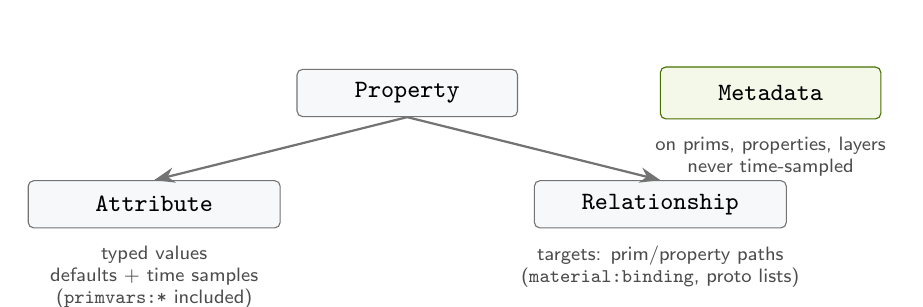
\begin{tikzpicture}[node distance=3mm and 6mm]
    \node[primbox, minimum width=2.8cm] (prop) {Property};
    \node[primbox, minimum width=3.2cm, below left=8mm and 2mm of prop] (attr) {Attribute};
    \node[primbox, minimum width=3.2cm, below right=8mm and 2mm of prop] (rel) {Relationship};
    \node[notetext, below=1mm of attr, align=center]
      {typed values\\defaults + time samples\\(\texttt{primvars:*} included)};
    \node[notetext, below=1mm of rel, align=center]
      {targets: prim/property paths\\(\texttt{material:binding}, proto lists)};
    \node[layerbox, right=18mm of prop, minimum width=2.8cm] (meta) {Metadata};
    \node[notetext, below=1mm of meta, align=center]
      {on prims, properties, layers\\never time-sampled};
    \draw[arc, draw=black!55] (prop.south) -- (attr.north);
    \draw[arc, draw=black!55] (prop.south) -- (rel.north);
  \end{tikzpicture}
  \caption{What can hold data in USD. The exam loves the boundaries: a
  time-varying value can never live in metadata; a path target can never live
  in an attribute.}
  \label{fig:prop-taxonomy}
\end{figure}

\subsection{Value types and roles}\label{sec:dm-types}\objref{5.2}
Sdf's type registry pairs storage with \emph{role}. Choosing well is an exam
objective in itself:

\begin{lstlisting}
#usda 1.0
( defaultPrim = "Props" )
def Scope "Props" {
    def Xform "Crate" {
        token visibility = "inherited"
        asset texture = @./wood.png@
        color3f[] primvars:displayColor = [(0.4, 0.25, 0.1)]
        matrix4d xformOp:transform = ( (1, 0, 0, 0), (0, 1, 0, 0),
                                       (0, 0, 1, 0), (0, 0, 0, 1) )
        uniform token[] xformOpOrder = ["xformOp:transform"]
        custom string notes = "hero prop"
        custom rel inspiration = </Props/Reference>
    }
    def Xform "Reference" {
    }
}
\end{lstlisting}

\noindent\texttt{token} is for closed vocabularies the runtime switches on
(\texttt{visibility} values); \texttt{asset} marks resolver-relevant paths;
the \texttt{color3f}, \texttt{point3f}, \texttt{normal3f}, and
\texttt{vector3f} roles tell consumers how to transform and color-manage
three floats;
\texttt{uniform} means ``not time-sampleable''; and a relationship ---
\texttt{rel} --- is the only correct way to say ``that prim over there''.
Figure~\ref{fig:propspanel} is this exact prim in usdview's property panel.

\begin{figure}[ht]
  \centering
  \begin{tikzpicture}
    \node[anchor=south west, inner sep=0] (img)
      {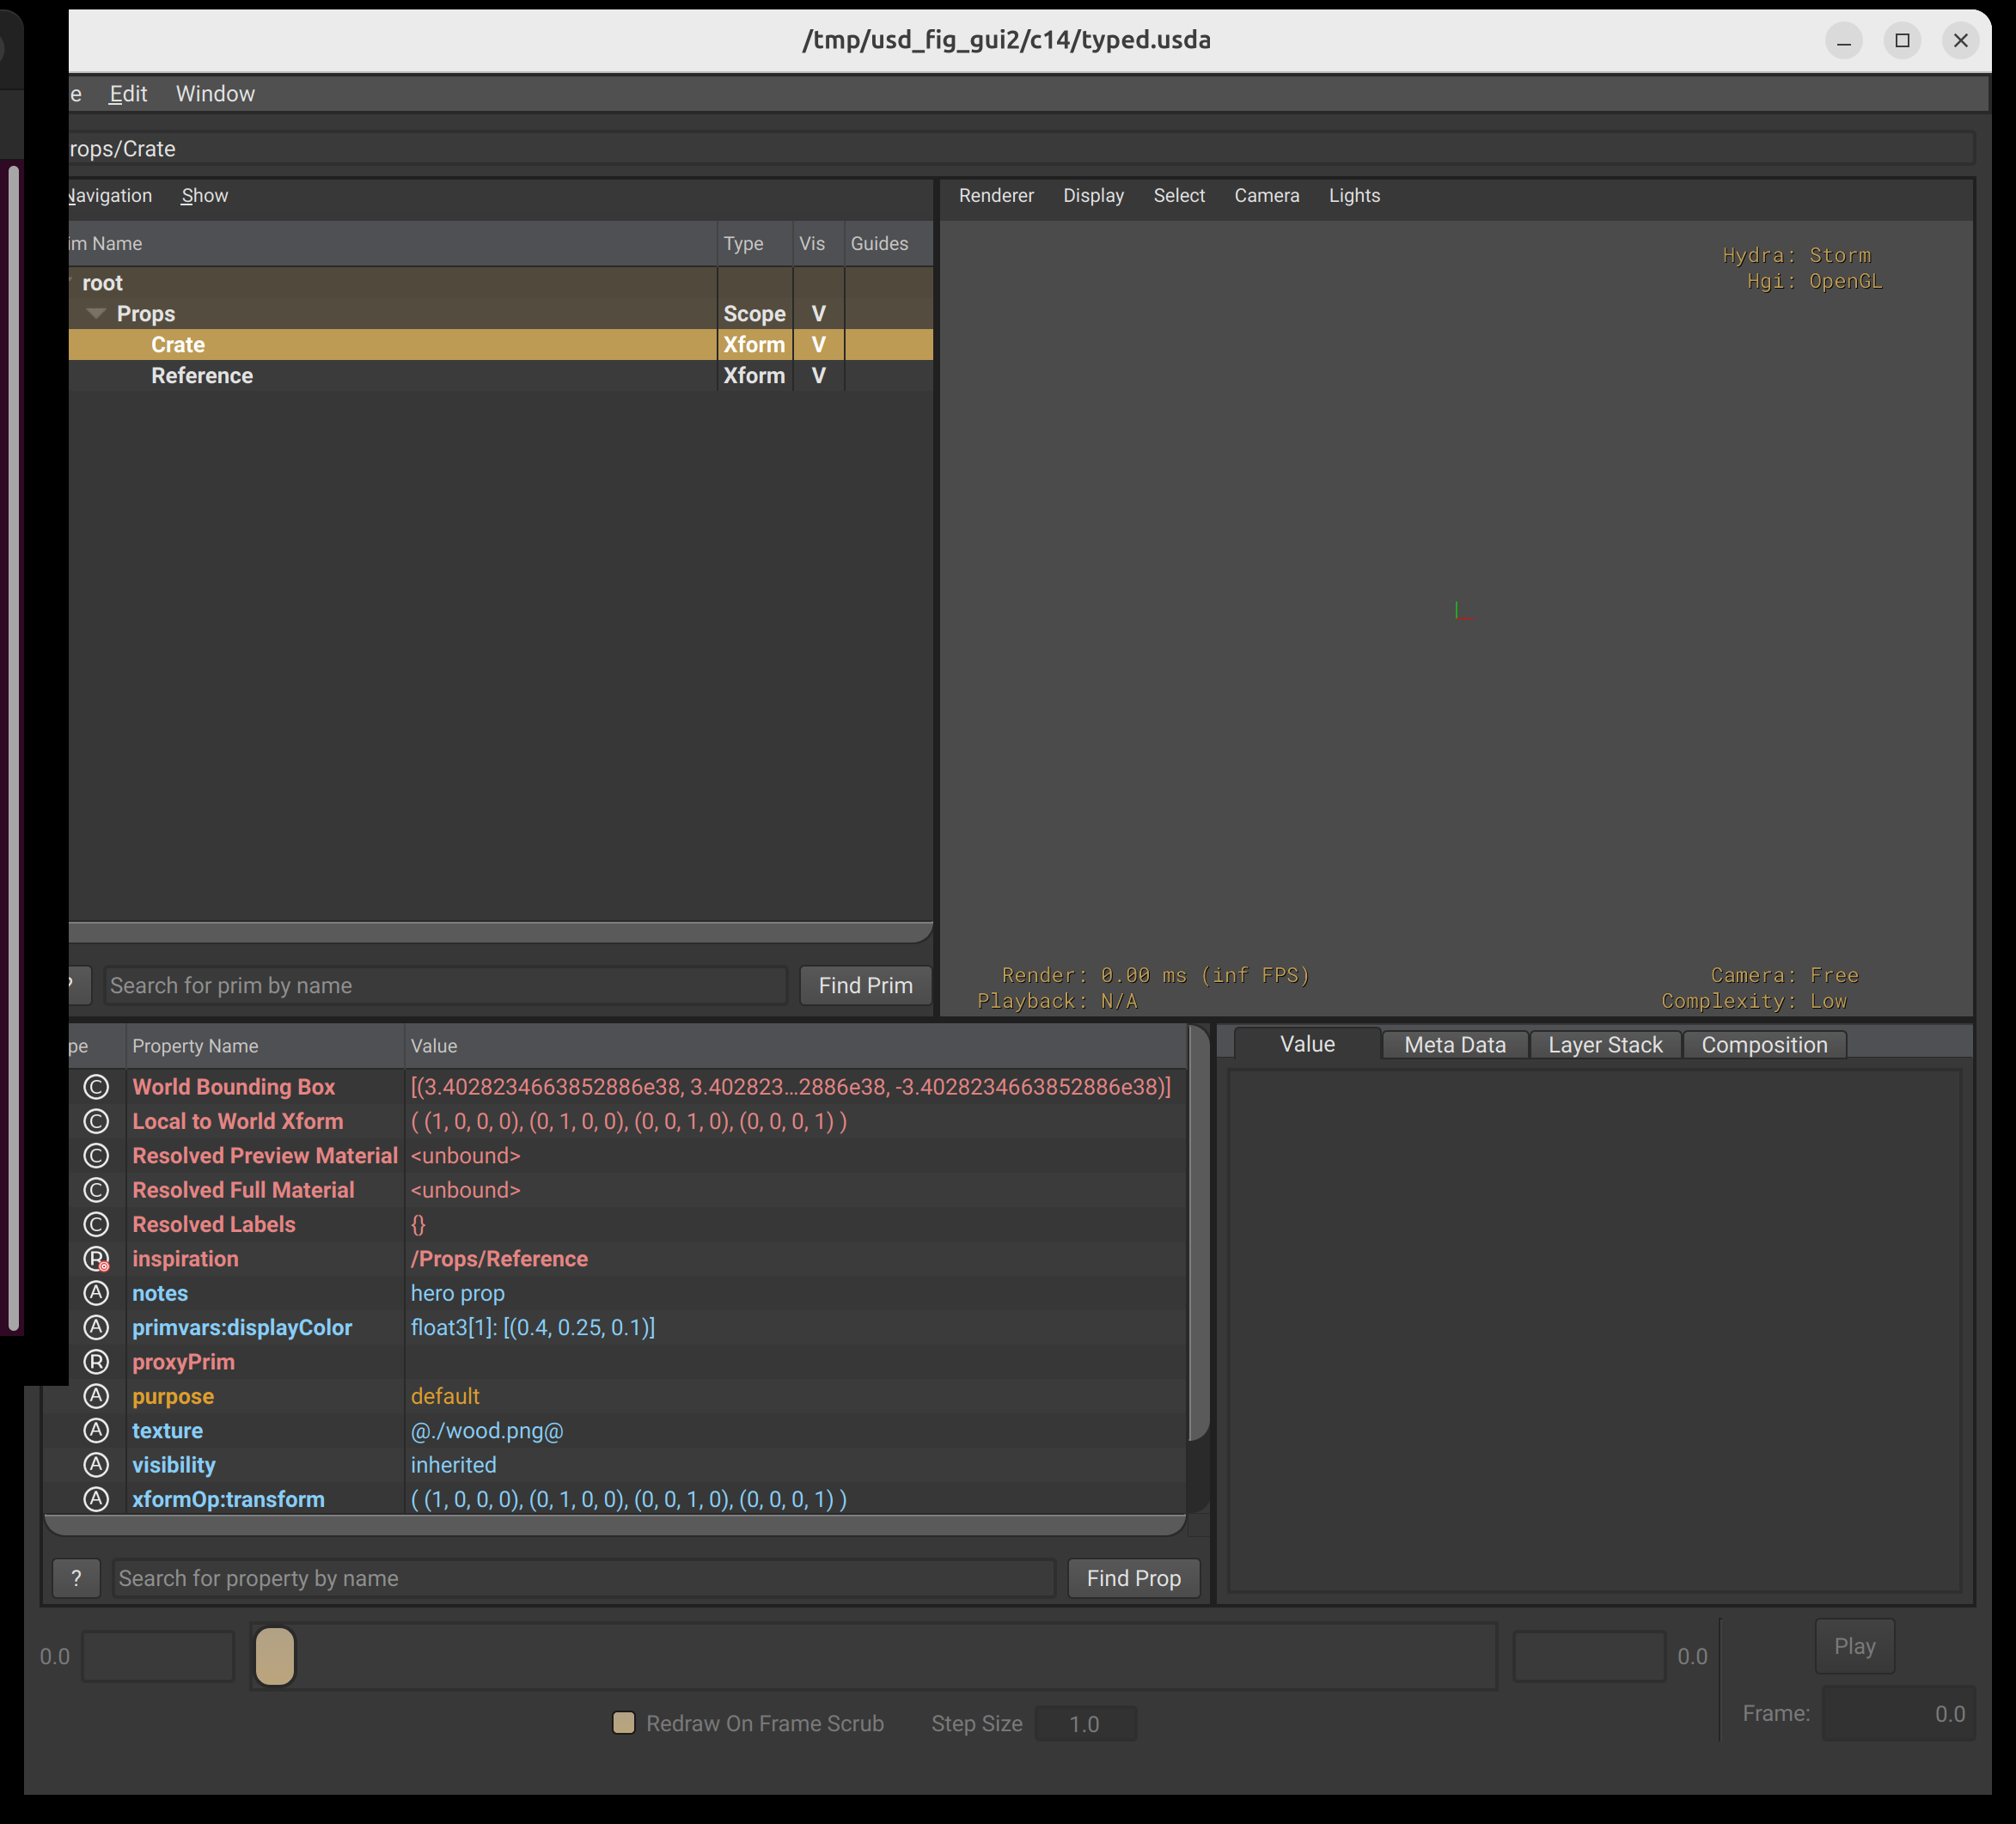
\includegraphics[trim={30 0 0 0}, clip, width=0.95\linewidth]{figures/c14_usdview_props.png}};
    \begin{scope}[x={(img.south east)}, y={(img.north west)}]
      \node[notetext, draw=arcRef, fill=white, rounded corners=1pt,
            text width=0.27\linewidth, align=left] (rel) at (0.74,0.37)
        {a relationship's ``value'' is a target path};
      \draw[refArc] (rel.west) -- (0.36,0.315);
      \node[notetext, draw=arcPay!85!black, fill=white, rounded corners=1pt,
            text width=0.27\linewidth, align=left] (ast) at (0.74,0.20)
        {asset-typed: quoted with \texttt{@...@}, visible to the resolver};
      \draw[payArc] (ast.west) -- (0.33,0.225);
    \end{scope}
  \end{tikzpicture}
  \caption{The type-zoo prim in usdview: every property displays its declared
  type and role --- \texttt{inspiration} resolves to a prim path,
  \texttt{texture} to an asset path, \texttt{primvars:displayColor} to a
  color array. Property retrieval, made visual.}
  \label{fig:propspanel}
\end{figure}

\subsection{Primvars and interpolation}\label{sec:dm-primvars}\objref{5.1, 8.1}
\index{primvar}\index{interpolation}A primvar is an attribute in the
\texttt{primvars:} namespace plus two superpowers: it \emph{inherits down
namespace} (constant primvars flow to descendants) and it carries
\emph{interpolation} --- how values map onto the surface:

\begin{lstlisting}
#usda 1.0
( defaultPrim = "Plate" )
def Mesh "Plate" {
    float3[] extent = [(-1, 0, -1), (1, 0, 1)]
    int[] faceVertexCounts = [4]
    int[] faceVertexIndices = [0, 1, 2, 3]
    point3f[] points = [(-1, 0, -1), (1, 0, -1), (1, 0, 1), (-1, 0, 1)]
    texCoord2f[] primvars:st = [(0, 0), (1, 0), (1, 1), (0, 1)] (
        interpolation = "faceVarying"
    )
    int[] primvars:st:indices = [0, 1, 2, 3]
}
\end{lstlisting}

\noindent Element-count rules: \emph{constant} = 1, \emph{uniform} = one per
face, \emph{vertex} = one per point, \emph{faceVarying} = one per
face-vertex (corner) --- with \texttt{:indices}, the rule applies to the
\emph{indices}, letting corners share values. UVs are typically
\texttt{primvars:st}, faceVarying, indexed.

\begin{Gotcha}
\objref{5.5, 6.4}``My render looks wrong'' is usually one of: interpolation whose element
count does not match the data (validator material!), \texttt{:indices}
pointing past the value array, a \texttt{vector3f} treated as a
\texttt{point3f} (translations apply to points, not vectors), or a stale
\texttt{extent} culling the mesh. All four are data bugs, not renderer bugs.
\end{Gotcha}

\subsection{Authoring and retrieving with the API}\label{sec:dm-api}\objref{5.1, 5.3, 5.4}
The same model drives the Python surface --- create a primvar, stash custom
metadata, list what a prim carries:

\begin{lstlisting}[language=Python]
from pxr import Sdf, Usd, UsdGeom

stage = Usd.Stage.CreateInMemory()
mesh = UsdGeom.Mesh.Define(stage, "/Crate")
prim = mesh.GetPrim()

wear = UsdGeom.PrimvarsAPI(prim).CreatePrimvar(
    "wear", Sdf.ValueTypeNames.Float, UsdGeom.Tokens.constant)
wear.Set(0.5)

prim.SetCustomDataByKey("studio:reviewed", True)

print(wear.GetName(), wear.Get(), wear.GetInterpolation())
# primvars:wear 0.5 constant
print(prim.GetCustomDataByKey("studio:reviewed"))   # True
print([a.GetName() for a in prim.GetAttributes() if a.IsAuthored()])
# ['primvars:wear']
\end{lstlisting}

\noindent Retrieval comes in layers of specificity:
\texttt{GetPropertyNames()} (everything), \texttt{GetAttributes()} /
\texttt{GetRelationships()} (by property kind),
\texttt{GetPropertiesInNamespace("primvars")} (by namespace), and schema
accessors (\texttt{GetPointsAttr()}) when you know the type.\index{customData}

\begin{ExamTip}
\texttt{customData} is the junk drawer --- free-form, ignored by the runtime.
\texttt{assetInfo} is for asset identity. If the data needs a \emph{type},
\emph{time samples}, or \emph{querying at scale}, it wants to be an
attribute (or a proper schema), not metadata.
\end{ExamTip}

\subsection{Keeping extent honest}\label{sec:dm-extent}\objref{5.6}
\index{extent}Whoever updates \texttt{points} owns \texttt{extent} --- the
exam states it as its own objective, and Sample Question 5 tests it:

\begin{lstlisting}[language=Python]
from pxr import Usd, UsdGeom

stage = Usd.Stage.Open("mesh_uv.usda")
mesh = UsdGeom.Mesh(stage.GetPrimAtPath("/Plate"))

points = [(x * 2, y * 2, z * 2) for x, y, z in mesh.GetPointsAttr().Get()]
mesh.GetPointsAttr().Set(points)

extent = UsdGeom.Boundable.ComputeExtentFromPlugins(
    mesh, Usd.TimeCode.Default())
mesh.GetExtentAttr().Set(extent)
print(extent)   # [(-2, 0, -2), (2, 0, 2)]
\end{lstlisting}

\subsection{Time, samples, and interpolation}\label{sec:dm-time}\objref{5.2, 5.5}
\index{timeSamples}\index{TimeCode}An attribute holds a \emph{default} and
optionally \emph{time samples}; queries take a \texttt{TimeCode}:

\begin{lstlisting}
#usda 1.0
( defaultPrim = "Ball" )
def Sphere "Ball" {
    double radius.timeSamples = {
        1: 1,
        11: 11,
    }
}
\end{lstlisting}

\begin{lstlisting}[language=Python]
from pxr import Usd

stage = Usd.Stage.Open("ball_anim.usda")
radius = stage.GetPrimAtPath("/Ball").GetAttribute("radius")

print(radius.Get(6))                       # 6.0  -- linear interpolation
print(radius.GetBracketingTimeSamples(6))  # (1.0, 11.0)

stage.SetInterpolationType(Usd.InterpolationTypeHeld)
print(radius.Get(6))                       # 1.0  -- held: previous sample
\end{lstlisting}

\noindent Three rules cover most exam traps: between samples, the
\emph{stage's} interpolation type decides (linear by default, held as an
option --- there is no spline yet); outside the sampled range the nearest
sample is held; and \texttt{Get()} with no argument means
\texttt{TimeCode.Default()}, which reads the \emph{default value, not the
samples} --- an attribute with only time samples returns nothing at Default.

\begin{Gotcha}
``The value is right in usdview but wrong in my script'' is often a
\texttt{TimeCode} bug: usdview queries at the current frame; your script
queried Default. Pass the time explicitly ---
\texttt{attr.Get(Usd.TimeCode(frame))} --- whenever samples exist.
\end{Gotcha}

\subsection{Transforms without tears: XformCommonAPI}\label{sec:dm-xform}\objref{5.1, 5.4}
\index{XformCommonAPI}\index{xformOp}Raw \texttt{xformOp:*} attributes are
flexible and easy to get wrong (op order!). For the standard
translate/rotate/scale case, \texttt{XformCommonAPI} authors a canonical
stack and reads it back as plain vectors:

\begin{lstlisting}[language=Python]
from pxr import Gf, Usd, UsdGeom

stage = Usd.Stage.CreateInMemory()
prim = UsdGeom.Xform.Define(stage, "/Crate").GetPrim()

api = UsdGeom.XformCommonAPI(prim)
api.SetTranslate(Gf.Vec3d(1, 2, 3))
api.SetRotate(Gf.Vec3f(0, 45, 0))
api.SetScale(Gf.Vec3f(2, 2, 2))

t, r, s, pivot, order = api.GetXformVectors(Usd.TimeCode.Default())
print(t, r, s)   # (1, 2, 3) (0, 45, 0) (2, 2, 2)
\end{lstlisting}

\noindent For world-space answers across a hierarchy, use
\texttt{UsdGeom.XformCache} --- it memoizes local-to-world matrices per time
code, which is also the right tool inside exporters.\index{XformCache}

\DrillsTitle
\subsection*{Drill 1: Primvar practice}
Write a minimal Mesh that includes \texttt{primvars:st} with faceVarying
interpolation.
\AnswerLines{10}
\begin{DrillSolution}
The chapter's Plate listing is the reference answer: counts/indices/points
for one quad, \texttt{texCoord2f[] primvars:st} with
\texttt{interpolation = "faceVarying"} in the attribute metadata, plus
\texttt{primvars:st:indices} so corners can share values. Bonus points in an
exam answer: authored \texttt{extent}.
\end{DrillSolution}

\subsection*{Drill 2: Type discipline}
Give 6 examples of common types (token, rel, float3, color3f[], matrix4d,
asset) and what you'd store in them.
\AnswerLines{8}
\begin{DrillSolution}
\texttt{token} --- closed vocabulary like \texttt{purpose = "proxy"};
\texttt{rel} --- ``points at'' data like \texttt{material:binding};
\texttt{float3}/\texttt{point3f}/\texttt{vector3f} --- positions vs
directions (role matters under transforms); \texttt{color3f[]} ---
\texttt{primvars:displayColor}; \texttt{matrix4d} ---
\texttt{xformOp:transform}; \texttt{asset} --- texture and layer paths the
resolver should see (never plain strings).
\end{DrillSolution}

\subsection*{Drill 3: Element-count audit}
A quad mesh (4 points, 1 face, 4 corners) has primvars with 1, 4, and 4
values. Which interpolations are legal for each?
\AnswerLines{6}
\begin{DrillSolution}
1 value $\Rightarrow$ constant. 4 values $\Rightarrow$ vertex (per point)
\emph{or} faceVarying (per corner --- this quad has exactly 4 corners), so
both are legal here; the distinction starts to matter the moment two faces
share a point. 4 values can never be uniform on a 1-face mesh (uniform needs
exactly 1).
\end{DrillSolution}

\section*{Checkpoint Questions}
\addcontentsline{toc}{section}{Checkpoint Questions}

\noindent\textbf{CQ1.} Where can a time-varying review note live: attribute
metadata, \texttt{customData}, or an attribute --- and why?
\begin{DrillSolution}
Only an attribute --- metadata (including \texttt{customData}) is never
time-sampled. If it varies over time, it is a value, and values live in
attributes.
\end{DrillSolution}

\noindent\textbf{CQ2.} \texttt{primvars:st} has 4 values,
\texttt{interpolation = "vertex"}, on a mesh with 6 points. What happens?
\begin{DrillSolution}
Element-count mismatch: vertex interpolation requires one value per point
(6). Renderers may drop the primvar, render garbage UVs, or warn --- the
asset is invalid even though it parses. This is exactly the class of
``unexpected visual results'' the exam asks you to diagnose.
\end{DrillSolution}

\noindent\textbf{CQ3.} After a tool doubles all \texttt{points}, the mesh
disappears in some views. Likely cause and fix?
\begin{DrillSolution}
Stale \texttt{extent}: bounds still describe the old size, so the camera or
renderer culls incorrectly. Recompute with
\texttt{ComputeExtentFromPlugins} and re-author \texttt{extent} --- the
chapter's listing is the fix, verbatim.
\end{DrillSolution}

\subsection*{Mini-checklist (tick when mastered)}
\begin{itemize}[leftmargin=*]
  \item[$\square$] I can place any datum: attribute vs relationship vs metadata.
  \item[$\square$] I can recite the four interpolations and their element counts.
  \item[$\square$] I know when \texttt{:indices} applies and what it changes.
  \item[$\square$] I re-author \texttt{extent} reflexively after touching \texttt{points}.
\end{itemize}

\DomainHeader{Debugging and Troubleshooting}{11\%}

\begin{Objectives}
  \item Recognize when \texttt{SdfChangeBlock} helps performance.
  \item Diagnose why opinions do not take effect on a composed stage.
  \item Resolve asset-management/path issues.
  \item Understand causes of unexpected visual results.
  \item Use diagnostics/profiling: TfDebug, diagnostic delegates, Trace,
        TfMallocTag, etc.
\end{Objectives}

\begin{Resources}
  \item Tutorials: \href{https://openusd.org/release/tut_inspect_and_author_props.html}{Inspecting and Authoring Properties}; \href{https://openusd.org/release/tut_traversing_stage.html}{Traversing a Stage}
  \item Tooling: \href{https://openusd.org/release/toolset.html#usdview}{\texttt{usdview}}
        (\href{https://docs.omniverse.nvidia.com/usd/latest/usdview/panel_composition.html#layer-stack}{Layer Stack / Composition tabs}),
        \href{https://openusd.org/release/toolset.html#usdcat}{\texttt{usdcat}}
  \item Technical references: USD FAQ \href{https://openusd.org/release/usdfaq.html#what-s-the-difference-between-an-over-and-a-typeless-def}{``Over vs Typeless Def''};
        \href{https://openusd.org/release/maxperf.html}{Maximizing USD Performance}
  \item OpenUSD API: \href{https://openusd.org/release/api/class_usd_property.html}{GetPropertyStack};
        \href{https://openusd.org/release/api/class_usd_stage.html}{UsdStage::MuteLayer};
        \href{https://openusd.org/release/api/class_usd_utils_coalescing_diagnostic_delegate.html}{UsdUtilsCoalescingDiagnosticDelegate};
        \href{https://openusd.org/release/api/class_sdf_change_block.html}{SdfChangeBlock}
\end{Resources}

\CheatSheetTitle
\begin{itemize}[leftmargin=*]
  \item \textbf{The three questions}, in order: Is my edit landing in the
        layer I think (edit target)? Is a stronger opinion winning (LIVRPS)?
        Is the prim composed at all (payload loaded, reference resolved,
        variant selected, \texttt{active})?\index{edit target}
  \item \textbf{Provenance tool \#1}:
        \texttt{attr.GetPropertyStack(time)} --- every opinion for a
        property, strongest first, with its layer.\index{GetPropertyStack}
  \item \textbf{Bisection tool \#1}: \texttt{stage.MuteLayer()} --- pull
        layers out of composition one at a time until the symptom
        disappears.\index{muting layers}
  \item \textbf{usdview} shows the same story interactively: Layer Stack and
        Composition tabs (see the Composition chapter's screenshot).
  \item \textbf{SdfChangeBlock}: batch many small authoring edits into one
        recomposition --- the fix for ``my exporter spends all its time in
        change processing''.\index{SdfChangeBlock}
  \item \textbf{TfDebug}: hundreds of runtime switches
        (\texttt{TF\_DEBUG=PLUG\_*}, \texttt{AR\_*}, \texttt{PCP\_*}) that
        print what plugins, resolvers, and composition are doing.\index{TfDebug}
  \item \textbf{Silence is a lie}: warnings on stderr --- unresolved assets,
        missing \texttt{defaultPrim} --- are composition errors in disguise;
        make pipelines fail on them.
\end{itemize}

\section{Core Concepts}

\subsection{Reproduce small, then interrogate}\label{sec:dbg-repro}\objref{6.2}
Every composition mystery shrinks to a few layers. This chapter's repro ---
one definition, one override, one stack:

\begin{lstlisting}
#usda 1.0
def Sphere "Ball" {
    double radius = 1
}
\end{lstlisting}

\begin{lstlisting}
#usda 1.0
over "Ball" {
    double radius = 3
}
\end{lstlisting}

\begin{lstlisting}
#usda 1.0
(
    subLayers = [@./lite.usda@, @./base.usda@]
)
\end{lstlisting}

\subsection{Who wins, and from where}\label{sec:dbg-stack}\objref{6.2}
The single most useful debugging call in USD answers ``where did this value
come from?'' --- every authored opinion for a property, strongest first:

\begin{lstlisting}[language=Python]
from pxr import Usd

stage = Usd.Stage.Open("shot.usda")
attr = stage.GetPrimAtPath("/Ball").GetAttribute("radius")
print(attr.Get())   # 3.0
for spec in attr.GetPropertyStack(Usd.TimeCode.Default()):
    print(spec.layer.GetDisplayName(), spec.default)
# lite.usda 3.0   <-- strongest first: this one wins
# base.usda 1.0
\end{lstlisting}

\noindent This is the scripted twin of usdview's Layer Stack tab ---
Figure~\ref{fig:layerstack} is the same investigation done interactively:
select the prim, open \emph{Layer Stack}, read the opinions strongest-first.
Same workflow for whole prims: \texttt{prim.GetPrimStack()}.

\begin{figure}[ht]
  \centering
  \begin{tikzpicture}
    \node[anchor=south west, inner sep=0] (img)
      {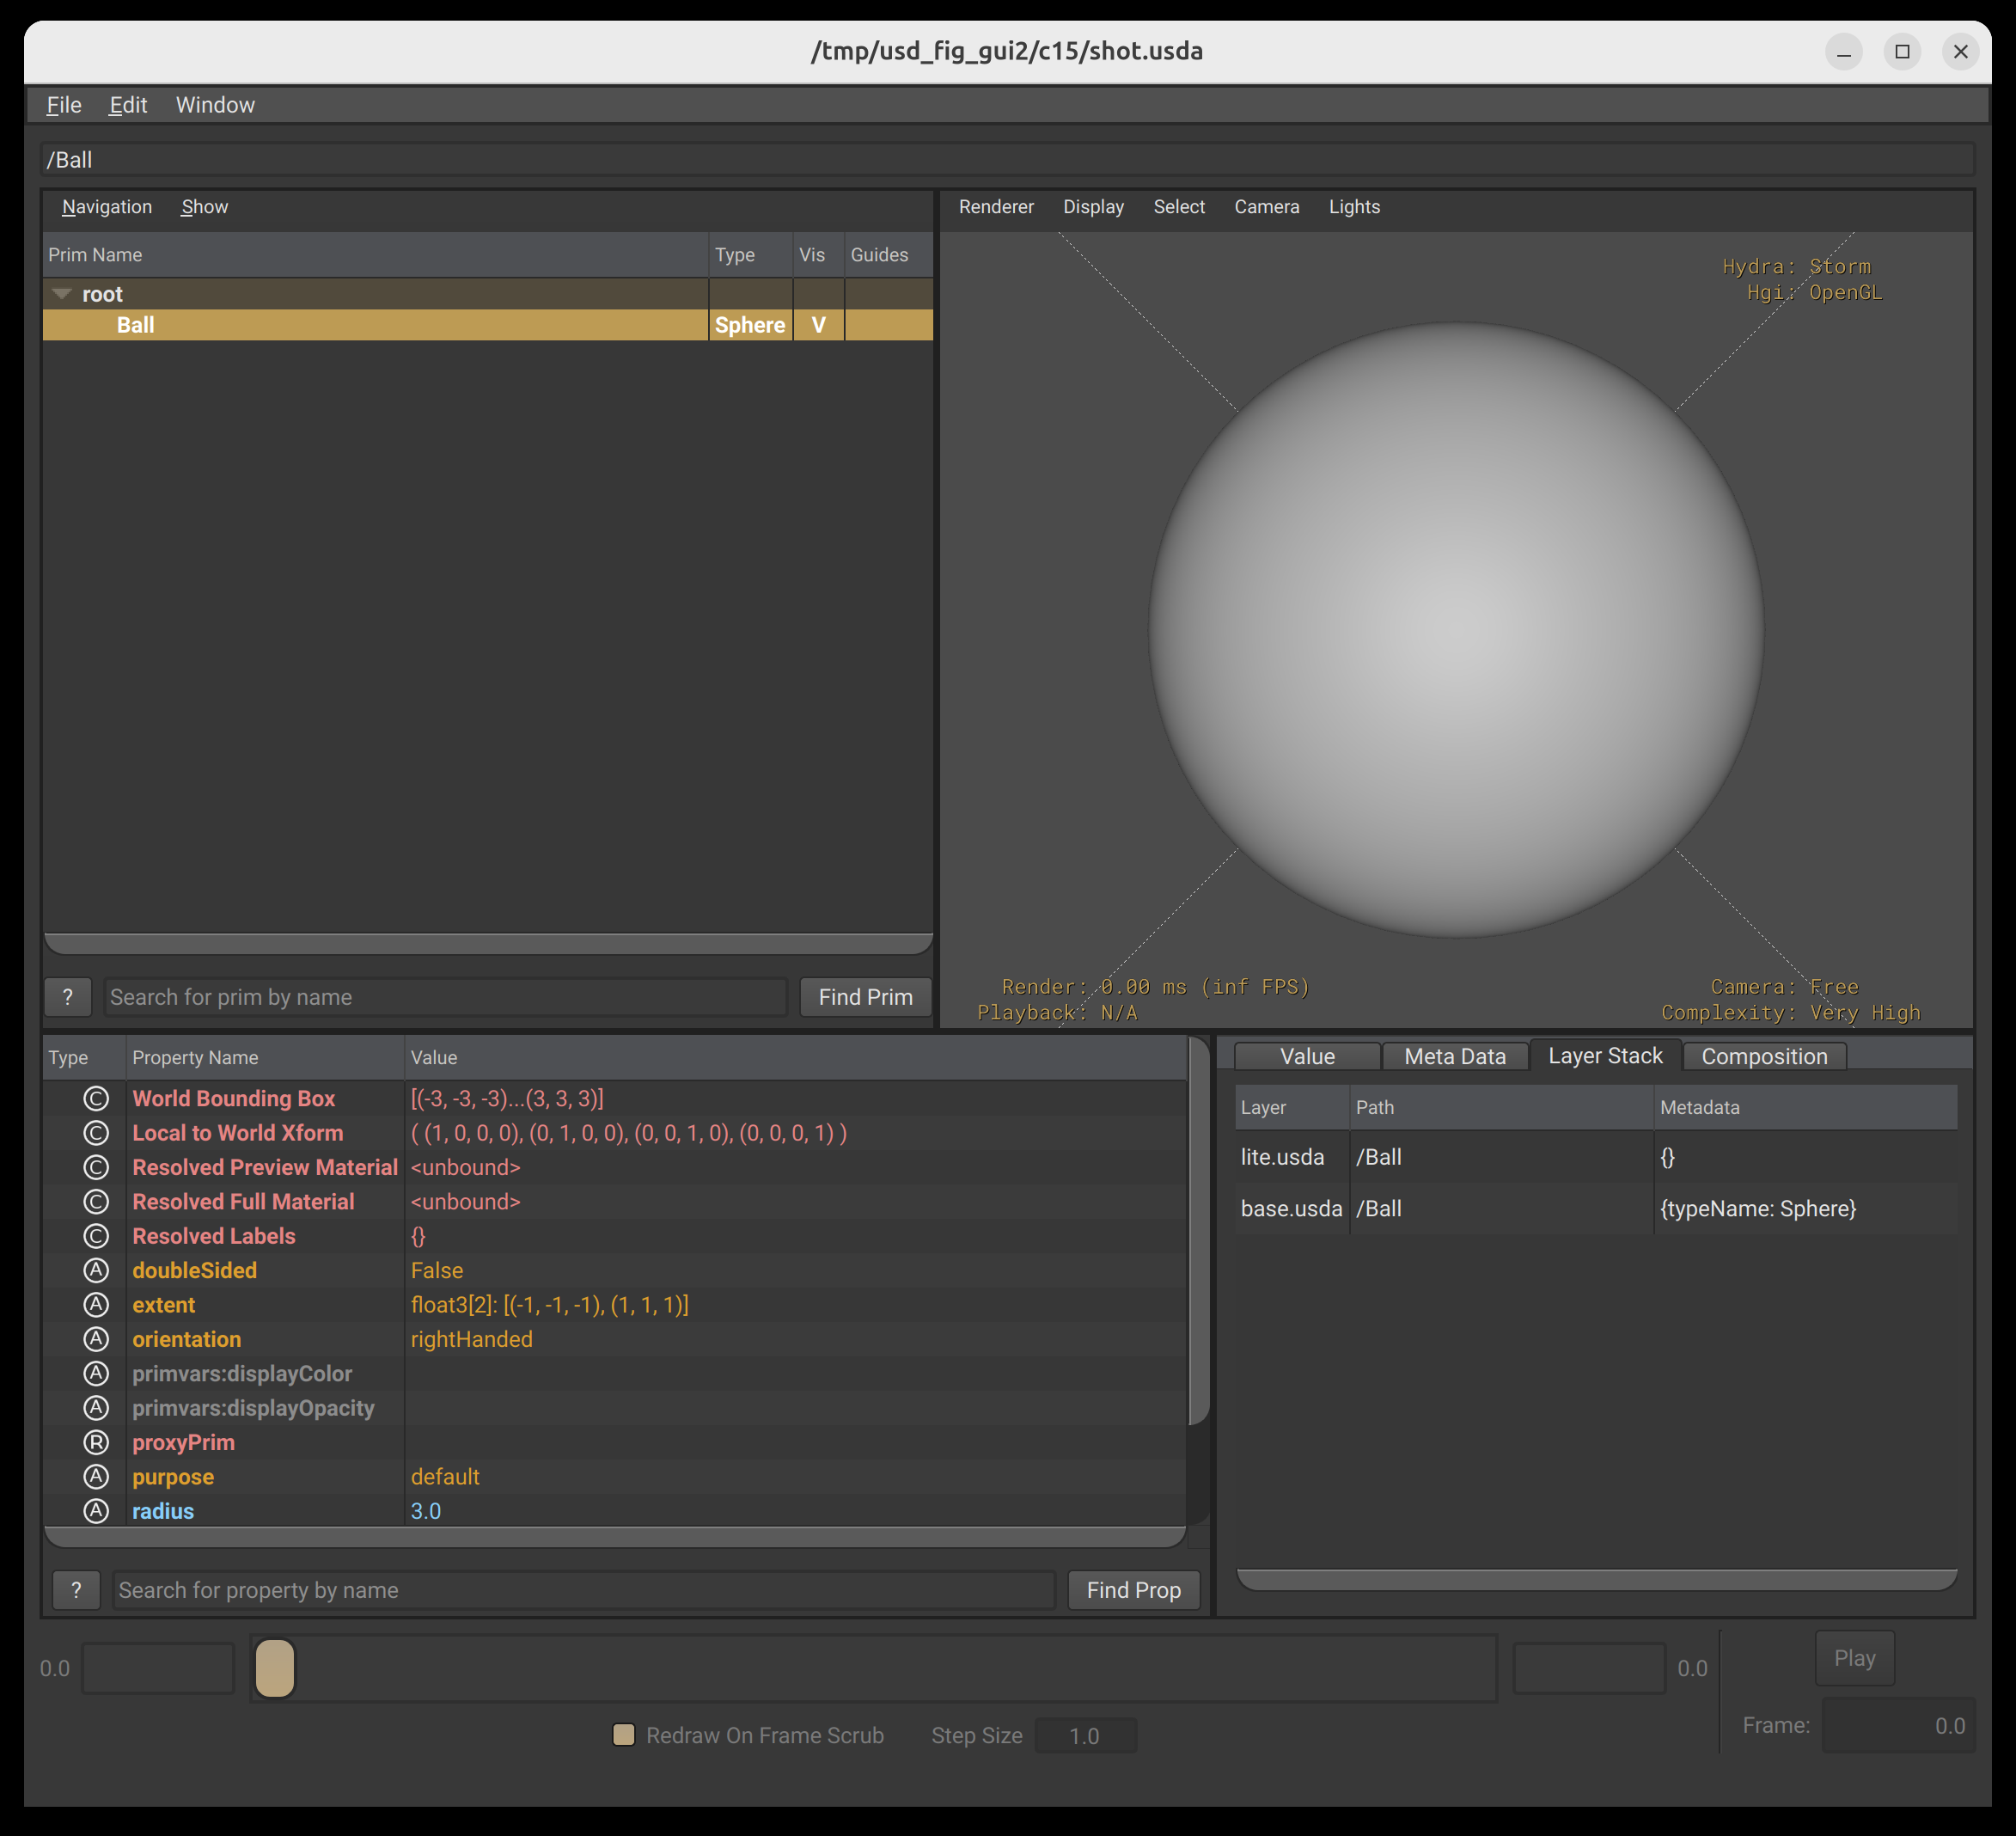
\includegraphics[width=0.95\linewidth]{figures/c15_usdview_layerstack.png}};
    \begin{scope}[x={(img.south east)}, y={(img.north west)}]
      \node[notetext, draw=arcVar, fill=white, rounded corners=1pt,
            text width=0.26\linewidth, align=left] (tab) at (0.46,0.50)
        {the \emph{Layer Stack} tab: every layer with an opinion on the
         selection};
      \draw[varArc] (tab.east) -- (0.755,0.43);
      \node[notetext, draw=usdgreen!60!black, fill=white, rounded corners=1pt,
            text width=0.26\linewidth, align=left] (rows) at (0.46,0.26)
        {\texttt{lite.usda} above \texttt{base.usda} --- strongest first,
         matching \texttt{GetPropertyStack}};
      \draw[subArc] (rows.east) -- (0.64,0.36);
    \end{scope}
  \end{tikzpicture}
  \caption{usdview on this chapter's repro with \texttt{/Ball} selected. The
  Layer Stack tab lists both contributing layers strongest-first; the
  property panel shows the winning \texttt{radius = 3.0}.}
  \label{fig:layerstack}
\end{figure}

\begin{ExamTip}
``Why doesn't my opinion take effect?'' has exactly four endings: a stronger
opinion (read the property stack top-down), the edit landed in the wrong
layer (check the edit target), the prim isn't fully composed (payload
unloaded, broken reference, wrong variant, \texttt{active = false}), or the
value never reached this property at all (typo: \texttt{over} on the wrong
path silently authors nothing useful --- see the ``over vs typeless def''
FAQ).
\end{ExamTip}

\subsection{Bisection: mute layers until the bug leaves}\label{sec:dbg-mute}\objref{6.2, 6.3}
\index{muting layers}When the property stack is deep, stop reading and start
cutting --- muting removes a layer from composition without touching files:

\begin{lstlisting}[language=Python]
from pxr import Sdf, Usd

stage = Usd.Stage.Open("shot.usda")
radius = stage.GetPrimAtPath("/Ball").GetAttribute("radius")
print(radius.Get())                       # 3.0 -- lite.usda wins

lite = Sdf.Layer.FindOrOpen("lite.usda")  # the suspect
stage.MuteLayer(lite.identifier)
print(radius.Get())                       # 1.0 -- base.usda shows through

stage.UnmuteLayer(lite.identifier)
\end{lstlisting}

\noindent The same bisection spirit applies to the working set
(\texttt{Load}/\texttt{Unload} payloads), variant selections, and
deactivating subtrees (\texttt{SetActive(False)}) --- isolate until the
symptom names its layer.

\subsection{Performance: batch your edits}\label{sec:dbg-perf}\objref{6.1}
\index{SdfChangeBlock}Every authoring call can trigger change processing and
recomposition; tools that author thousands of opinions one-by-one spend
their life there. \texttt{SdfChangeBlock} batches Sdf-level edits into a
single notification:

\begin{lstlisting}[language=Python]
from pxr import Sdf

layer = Sdf.Layer.CreateAnonymous()
with Sdf.ChangeBlock():
    for i in range(100):
        prim = Sdf.CreatePrimInLayer(layer, f"/Props/Prop_{i:03}")
        prim.specifier = Sdf.SpecifierDef
        prim.typeName = "Xform"
print(len(layer.GetPrimAtPath("/Props").nameChildren))   # 100
\end{lstlisting}

\begin{Gotcha}
Inside a change block, work at the \emph{Sdf} level and do not read back
through Usd APIs --- composition is intentionally stale until the block
closes. The objective is literally ``recognize \emph{when} SdfChangeBlock
helps'': many small edits, one recomposition. It does not make a single big
edit faster.
\end{Gotcha}

\subsection{Diagnostics: make USD tell you}\label{sec:dbg-diag}\objref{6.5}
\index{TfDebug}USD ships with runtime debug switches --- no rebuild, just an
environment variable: \texttt{TF\_DEBUG=PLUG\_REGISTRATION} (why isn't my
plugin loading?), \texttt{AR\_RESOLVER\_INIT} (which resolver am I using?),
\texttt{USD\_CHANGES} / \texttt{PCP\_CHANGES} (what is recomposing, and
why?). Discover them from Python:

\begin{lstlisting}[language=Python]
from pxr import Tf

names = Tf.Debug.GetDebugSymbolNames()
print(len(names) > 0)                              # True
print("USD_CHANGES" in names, "PLUG_REGISTRATION" in names)  # True True
# enable from code: Tf.Debug.SetDebugSymbolsByName("USD_CHANGES", True)
\end{lstlisting}

\noindent For floods of warnings, a \emph{coalescing diagnostic delegate}
(in \texttt{UsdUtils}; see Resources) collects and deduplicates them instead
of spamming stderr.

For \emph{time}, the \texttt{Trace} module instruments scopes and prints a
nested timing tree --- this runs anywhere USD runs, no rebuild:

\begin{lstlisting}[language=Python]
from pxr import Trace, Usd

collector = Trace.Collector()
collector.enabled = True
with Trace.TraceScope("open-and-traverse"):
    stage = Usd.Stage.Open("shot.usda")
    count = len(list(stage.Traverse()))
collector.enabled = False

Trace.Reporter.globalReporter.Report()
# Main Thread
#  | open-and-traverse
#  |   UsdStage::Open
#  |   ...inclusive/exclusive ms per scope...
\end{lstlisting}

\noindent Your named scope appears among USD's own (the \texttt{Pcp}
prim-indexing scopes and friends), so ``where does opening this stage spend
its time'' stops being a guess. For memory, \texttt{TfMallocTag}
plays the same role on allocations.\index{Trace} For time, the \texttt{Trace} module
instruments scopes (\texttt{usdview} ships a built-in profiler view); for
memory, \texttt{TfMallocTag} attributes allocations --- both are ``know they
exist and what for'' exam material.\index{Trace}\index{TfMallocTag}

\begin{figure}[ht]
  \centering
  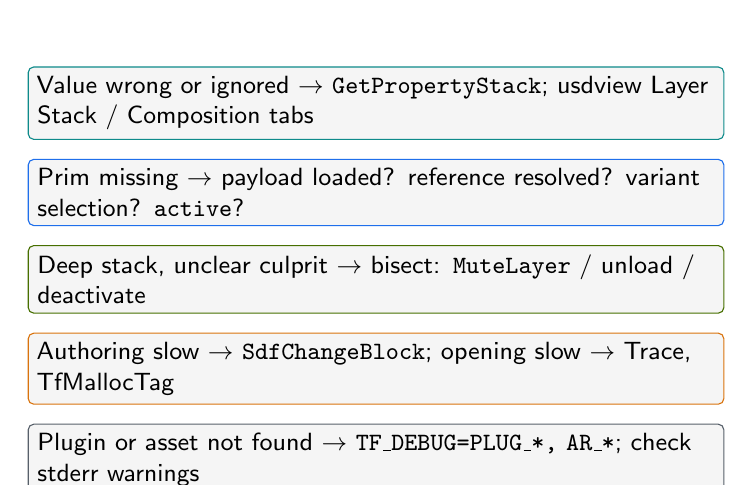
\begin{tikzpicture}[node distance=2.4mm]
    \node[strengthbox, draw=arcVar]  (s1)
      {Value wrong or ignored $\rightarrow$ \texttt{GetPropertyStack}; usdview Layer Stack / Composition tabs};
    \node[strengthbox, draw=arcRef, below=of s1]  (s2)
      {Prim missing $\rightarrow$ payload loaded? reference resolved? variant selection? \texttt{active}?};
    \node[strengthbox, draw=usdgreen!60!black, below=of s2] (s3)
      {Deep stack, unclear culprit $\rightarrow$ bisect: \texttt{MuteLayer} / unload / deactivate};
    \node[strengthbox, draw=arcPay, below=of s3] (s4)
      {Authoring slow $\rightarrow$ \texttt{SdfChangeBlock}; opening slow $\rightarrow$ Trace, TfMallocTag};
    \node[strengthbox, draw=arcSpec, below=of s4] (s5)
      {Plugin or asset not found $\rightarrow$ \texttt{TF\_DEBUG=PLUG\_*, AR\_*}; check stderr warnings};
  \end{tikzpicture}
  \caption{Symptom $\rightarrow$ tool. Start at the top; each row is cheaper
  than guessing.}
  \label{fig:debug-tree}
\end{figure}

\DrillsTitle
\subsection*{Drill 1: Three-step diagnosis}
Write your personal 3-step flow for ``why didn't my value apply?''
\AnswerLines{8}
\begin{DrillSolution}
(1) \emph{Where did my edit go?} --- check the edit target / which layer
gained the opinion. (2) \emph{Who wins?} --- \texttt{GetPropertyStack} or
usdview's Composition tab; read LIVRPS top-down. (3) \emph{Is it composed at
all?} --- payload load state, reference resolution warnings, variant
selection, \texttt{active}. Three questions, three tools, no guessing.
\end{DrillSolution}

\subsection*{Drill 2: Path failure taxonomy}
List 5 common reasons asset paths fail in production (and what fixes them).
\AnswerLines{8}
\begin{DrillSolution}
(1) Absolute, machine-specific paths $\Rightarrow$ publish gate enforcing
relative paths. (2) Backslashes from Windows exports $\Rightarrow$ normalize
at export. (3) Path resolves differently on the farm $\Rightarrow$ resolver
context/config parity; \texttt{TF\_DEBUG=AR\_*} to see resolution. (4)
Missing \texttt{defaultPrim} in the referenced layer $\Rightarrow$ the
reference resolves the file but composes nothing. (5) Case mismatch on
case-sensitive filesystems $\Rightarrow$ naming convention + validator.
\end{DrillSolution}

\subsection*{Drill 3: ChangeBlock judgment}
For each, does \texttt{SdfChangeBlock} help? (a) importer creating 10{,}000
prims; (b) setting one attribute; (c) a tool that authors then immediately
reads composed values in a loop.
\AnswerLines{6}
\begin{DrillSolution}
(a) Yes --- the canonical case: thousands of edits, one recomposition.
(b) No --- nothing to batch. (c) No --- worse than no: reads inside the
block see stale composition; restructure to write-all-then-read.
\end{DrillSolution}

\section*{Checkpoint Questions}
\addcontentsline{toc}{section}{Checkpoint Questions}

\noindent\textbf{CQ1.} In this chapter's repro, what does
\texttt{GetPropertyStack} print, and what does the \emph{order} mean?
\begin{DrillSolution}
\texttt{lite.usda 3.0} then \texttt{base.usda 1.0} --- strongest first.
The top entry is the opinion the stage returns; everything below is what
would win if the entries above disappeared (which \texttt{MuteLayer}
demonstrates: mute \texttt{lite.usda} and the value falls back to 1.0).
\end{DrillSolution}

\noindent\textbf{CQ2.} A TD reports the stage ``randomly recomposes'' during
their tool's run, making it slow. Which two facilities do you reach for?
\begin{DrillSolution}
\texttt{TF\_DEBUG=USD\_CHANGES} / \texttt{PCP\_CHANGES} to see \emph{what}
changes and why, and \texttt{SdfChangeBlock} around the tool's authoring
loop so the many small edits coalesce into one recomposition.
\end{DrillSolution}

\noindent\textbf{CQ3.} The stage opens, the render is fine, but stderr shows
``Unresolved reference prim path \ldots\ \texttt{<defaultPrim>}''. Why must
this fail the publish anyway?
\begin{DrillSolution}
The reference composed \emph{nothing} --- the stage merely survived. The
missing content (or the missing \texttt{defaultPrim} in the target layer)
will surface downstream where it is harder to trace. Warnings on stderr are
composition errors in disguise; pipelines treat them as failures.
\end{DrillSolution}

\subsection*{Mini-checklist (tick when mastered)}
\begin{itemize}[leftmargin=*]
  \item[$\square$] I ask the three questions in order before touching code.
  \item[$\square$] I can read a property stack and name the winning layer.
  \item[$\square$] I bisect with mute/unload/deactivate instead of guessing.
  \item[$\square$] I know which TF\_DEBUG families exist and when to flip them.
\end{itemize}

\DomainHeader{Pipeline Development}{14\%}

\begin{Objectives}
  \item Convert USD to common formats and ensure fidelity.
  \item Document asset structure guidelines.
  \item Explain USDC vs USDA trade-offs.
  \item Implement round-trip pipelines between DCC and USD.
  \item Integrate custom resolvers to manage asset paths.
  \item Represent custom metadata.
  \item Validate asset paths are formatted correctly.
  \item Write or extend a USD importer in a DCC.
\end{Objectives}

\begin{Resources}
  \item Learn OpenUSD: \href{https://docs.nvidia.com/learn-openusd/latest/asset-structure/index.html}{Asset Structure Principles and Content Aggregation};
        \href{https://docs.nvidia.com/learn-openusd/latest/composition-basics/index.html}{Composition Basics};
        \href{https://docs.nvidia.com/learn-openusd/latest/beyond-basics/index.html}{Beyond the Basics}
  \item Technical references: \href{https://docs.omniverse.nvidia.com/usd/latest/learn-openusd/independent/asset-structure-principles.html}{Principles of Scalable Asset Structure};
        \href{https://github.com/usd-wg/assets/blob/main/docs/asset-structure-guidelines.md}{ASWF Asset Structure Guidelines};
        USD FAQ \href{https://openusd.org/release/usdfaq.html#i-have-some-layers-i-want-to-combine-should-i-use-sublayers-or-references}{``SubLayers or References?''}
  \item OpenUSD glossary: \href{https://openusd.org/release/glossary.html#usdglossary-subcomponent}{Subcomponent}; \href{https://openusd.org/release/glossary.html#crate-file-format}{Crate File Format}; \href{https://openusd.org/release/glossary.html#flatten}{Flatten}; \href{https://openusd.org/release/glossary.html#edittarget}{Edit Target}
  \item OpenUSD API: \href{https://openusd.org/release/api/class_usd_stage.html}{UsdStage::Flatten};
        \href{https://openusd.org/release/api/class_sdf_change_block.html}{SdfChangeBlock};
        \href{https://openusd.org/release/api/class_usd_notice.html}{UsdNotice}
\end{Resources}

\CheatSheetTitle
\begin{itemize}[leftmargin=*]
  \item \textbf{Asset interface pattern}: a small entry-point layer (stable
        name, \texttt{defaultPrim}, \texttt{kind}, \texttt{assetInfo})
        payloads the heavy contents. Consumers reference the interface and
        never see the internals.\index{asset structure}
  \item \textbf{Kinds nest}: \texttt{assembly} $>$ \texttt{group} $>$
        \texttt{component} $>$ \texttt{subcomponent}; models must form a
        \emph{contiguous} tree --- a component under a plain prim is not a
        model.\index{kind}\index{model hierarchy}
  \item \textbf{SubLayers vs References}: layers in the same stack share one
        namespace (departments on a shot); references graft subtrees under
        new paths (assets into scenes).
  \item \textbf{Custom metadata}: per-asset facts in \texttt{assetInfo};
        free-form notes in \texttt{customData}; neither is time-sampled.
  \item \textbf{Asset paths}: relative, forward slashes, resolver-friendly ---
        validate at publish time, not when a render farm machine fails.
  \item \textbf{Resolvers} (Ar) turn logical identifiers
        (\texttt{asset://chair}) into real files --- pipelines pin versions
        there, not in scene files.\index{resolver}
  \item \textbf{Delivery}: flatten (and \texttt{usdzip}) to strip composition
        and proprietary paths from outgoing assets.
\end{itemize}

\section{Core Concepts}

\subsection{The asset interface pattern}\label{sec:pd-iface}\objref{7.2}
Scalable pipelines standardize what an asset looks like \emph{from outside}:
one small entry-point layer with a stable prim name and metadata, which
payloads the actual contents. Publishing a new version means updating what
the interface points at --- no consumer scene changes.

\begin{lstlisting}
#usda 1.0
( defaultPrim = "Chair" )
def Xform "Chair" (
    kind = "component"
    assetInfo = {
        string name = "Chair"
        string version = "v003"
    }
    prepend payload = @./contents.usda@
)
{
}
\end{lstlisting}

\begin{lstlisting}
#usda 1.0
( defaultPrim = "Chair" )
def Xform "Chair" {
    def Scope "Geometry" {
        def Sphere "Seat" {
        }
    }
    def Scope "Looks" {
    }
}
\end{lstlisting}

\noindent\objref{7.6}Everything heavy lives behind the payload: consumers
who only need the scene skeleton load nothing, and
\texttt{assetInfo}\index{assetInfo} carries pipeline facts (name, version)
that tools can query without conventions-by-folklore.

\begin{figure}[ht]
  \centering
  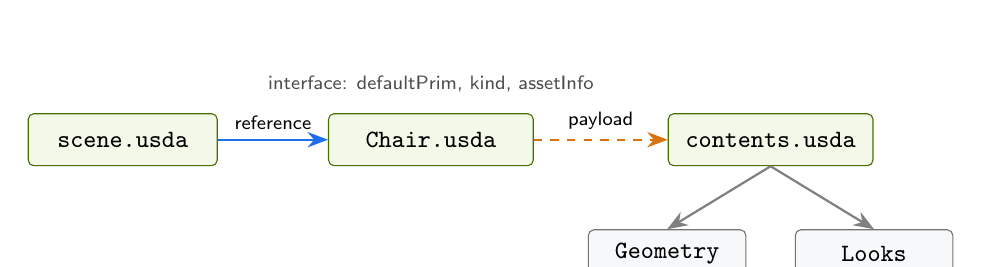
\begin{tikzpicture}
    \node[layerbox, minimum width=2.6cm] (iface) {Chair.usda};
    \node[notetext, above=1.5mm of iface] {interface: defaultPrim, kind, assetInfo};
    \node[layerbox, minimum width=2.6cm, right=17mm of iface] (contents) {contents.usda};
    \node[primbox, minimum width=2.0cm, below left=8mm and -10mm of contents] (geo) {Geometry};
    \node[primbox, minimum width=2.0cm, below right=8mm and -10mm of contents] (looks) {Looks};
    \draw[payArc] (iface) -- node[arcLabel] {payload} (contents);
    \draw[arc, draw=black!50] (contents.south) -- (geo.north);
    \draw[arc, draw=black!50] (contents.south) -- (looks.north);
    \node[layerbox, minimum width=2.4cm, left=14mm of iface] (scene) {scene.usda};
    \draw[refArc] (scene) -- node[arcLabel] {reference} (iface);
  \end{tikzpicture}
  \caption{The asset interface pattern: scenes reference a thin, stable entry
  point; the entry point payloads the heavy, evolving contents.}
  \label{fig:asset-iface}
\end{figure}

\subsection{Kinds and the model hierarchy}\label{sec:pd-kinds}\objref{7.2, 3.3}
\index{kind}\index{model hierarchy}Kinds make large scenes navigable:
\texttt{assembly} (published groups of models), \texttt{group} (organizational
interior nodes), \texttt{component} (the leaf-level publishable asset),
\texttt{subcomponent} (named pieces inside a component). Tools rely on the
\emph{model hierarchy rule}: every ancestor of a model must itself be a group
(or assembly). Break the chain and queries silently stop seeing your asset:

\begin{lstlisting}
#usda 1.0
( defaultPrim = "City" )
def Xform "City" ( kind = "assembly" ) {
    def Xform "Block" ( kind = "group" ) {
        def Xform "Bldg" ( kind = "component" ) {
            def Xform "Door" ( kind = "subcomponent" ) {
            }
        }
    }
    def Xform "Plain" {
        def Xform "Orphan" ( kind = "component" ) {
        }
    }
}
\end{lstlisting}

\begin{lstlisting}[language=Python]
from pxr import Usd

stage = Usd.Stage.Open("hierarchy.usda")
for path in ("/City", "/City/Block", "/City/Block/Bldg",
             "/City/Block/Bldg/Door", "/City/Plain/Orphan"):
    prim = stage.GetPrimAtPath(path)
    print(path, Usd.ModelAPI(prim).GetKind(),
          "model" if prim.IsModel() else "-")
\end{lstlisting}

\begin{Gotcha}
Run it (the book did): \texttt{/City/Plain/Orphan} has
\texttt{kind = component} yet \texttt{IsModel()} is \textbf{False} --- its
parent \texttt{Plain} has no group kind, so the model chain is broken.
Model-hierarchy traversals and ``find all components'' tools will skip it.
The fix is organizational, not code: give interior prims group kinds.
\end{Gotcha}

\subsection{SubLayers or references?}\label{sec:pd-subref}\objref{1.3, 1.5}
The FAQ question is an exam question in disguise. \emph{Sublayers} stack whole
layers into one shared namespace --- right when several parties author
opinions about the \emph{same} prims (shot workflows: layout, animation,
lighting). \emph{References} graft a subtree under a chosen path --- right
when content must appear (possibly many times) \emph{inside} something else
(assets into sets, sets into shots). A useful tiebreaker: if you would need to
re-path prims to combine the files, you wanted a reference.

\subsection{Validating asset paths}\label{sec:pd-paths}\objref{7.7}
\index{asset path}Published layers travel: farm machines, other sites, other
studios. Absolute paths and backslashes are how assets die in transit. The
dependency list is one call away, so gate it at publish:

\begin{lstlisting}[language=Python]
from pxr import Sdf

layer = Sdf.Layer.FindOrOpen("Chair.usda")
for path in layer.GetCompositionAssetDependencies():
    ok = not path.startswith("/") and "\\" not in path
    print(("OK  " if ok else "BAD ") + path)
# prints: OK  ./contents.usda
\end{lstlisting}

\begin{ExamTip}
``Validate asset paths are formatted correctly'' $\Rightarrow$ relative to the
layer, forward slashes, resolvable by the studio resolver, and no machine-
or user-specific roots. Pair it with the export validator from the Data
Exchange chapter --- same gate, same publish step.
\end{ExamTip}

\subsection{Resolvers in the pipeline}\label{sec:pd-res}\objref{7.5, 3.5}
\index{resolver}An Ar resolver maps \emph{logical} asset identifiers to real
files at open time: \texttt{asset://props/chair} might resolve to
\texttt{/site/v003/chair.usdc} today and to a new version tomorrow ---
without touching a single scene file. That is where pinning, platform roots,
and site-specific storage belong. Scene files keep clean logical paths; the
resolver owns policy. (Writing one is plugin work --- see Customizing USD.)

\subsection{Delivery: flatten and strip}\label{sec:pd-deliver}\objref{1.9, 7.1}
To send an asset outside the pipeline, remove what outsiders cannot resolve:
\texttt{UsdStage::Flatten()} bakes composition (and resolves internal
references away); \texttt{usdzip} packages the result with its textures.
What you lose --- overridability, variants, payload deferral --- is exactly
what you do not want to leak.\index{flatten}\index{usdzip}

\begin{DeepDive}
Asset-structure \emph{guidelines} (objective: document them!) are a short
contract, not a wiki: entry-point naming, \texttt{defaultPrim} == asset name,
kind policy, where Geometry/Looks scopes live, primvar and namespace
conventions, path rules, and the validation gate that enforces all of it.
The ASWF Asset Structure Guidelines are the public reference point --- steal
their shape.
\end{DeepDive}

\DrillsTitle
\subsection*{Drill 1: Asset contract}
Write 10 rules for your ``publishable USD asset contract''.
\AnswerLines{10}
\begin{DrillSolution}
A solid contract: (1) entry-point layer named like the asset; (2)
\texttt{defaultPrim} set and equal to the root prim; (3) root prim
\texttt{kind = component} (or assembly for published groups); (4) heavy data
behind a payload; (5) \texttt{Geometry}/\texttt{Looks} scopes in fixed
places; (6) \texttt{assetInfo} carries name and version; (7) all asset paths
relative with forward slashes; (8) units and up-axis declared; (9) extents
authored on all Boundables; (10) passes the publish validator --- no
warnings, \texttt{usdchecker} clean.
\end{DrillSolution}

\subsection*{Drill 2: Naming and layout}
Propose a directory structure for an asset with geo, materials, and anim.
\AnswerLines{8}
\begin{DrillSolution}
One workable shape: \texttt{Chair/Chair.usda} (interface),
\texttt{Chair/contents.usda} (assembly of the parts), and
\texttt{Chair/parts/\{geometry,looks,anim\}.usda}. The interface payloads
\texttt{contents.usda}; contents sublayers (same namespace!) the parts.
Versioning happens by publishing new part files and re-pointing ---
consumers only ever reference \texttt{Chair/Chair.usda}.
\end{DrillSolution}

\subsection*{Drill 3: SubLayers or references?}
For each case pick one and justify: (a) lighting overrides on a shot; (b) a
chair placed 40 times in a restaurant; (c) merging two departments' edits to
the same character.
\AnswerLines{6}
\begin{DrillSolution}
(a) Sublayer --- same namespace, strength by list order. (b) References
(instanceable!) --- the same subtree grafted under 40 paths. (c) Sublayers
--- both edit the same prims; references would duplicate the character under
two roots.
\end{DrillSolution}

\section*{Checkpoint Questions}
\addcontentsline{toc}{section}{Checkpoint Questions}

\noindent\textbf{CQ1.} A tool that lists all components in a scene misses one
asset. Its kind is correctly \texttt{component}. What is the first thing to
check?
\begin{DrillSolution}
The ancestors: model hierarchy must be contiguous. If any ancestor lacks a
group/assembly kind, \texttt{IsModel()} is False for the component and
model-hierarchy traversals skip it --- verified in this chapter's listing.
\end{DrillSolution}

\noindent\textbf{CQ2.} Publishing v004 of an asset must not touch any of the
1{,}200 shots referencing it. Which two mechanisms make that possible?
\begin{DrillSolution}
The asset interface pattern (shots reference a stable entry-point layer, so
content behind it can change) and/or a resolver that maps a logical
identifier to the current published version. Both keep ``which version''
out of scene files.
\end{DrillSolution}

\noindent\textbf{CQ3.} Name the API call that lists a layer's external asset
dependencies for a path-validation gate.
\begin{DrillSolution}
\texttt{Sdf.Layer.GetCompositionAssetDependencies()} --- sublayer, reference,
and payload asset paths of that layer, ready to be checked for absolute
paths, backslashes, and resolvability.
\end{DrillSolution}

\subsection*{Mini-checklist (tick when mastered)}
\begin{itemize}[leftmargin=*]
  \item[$\square$] I can draw the asset interface pattern from memory.
  \item[$\square$] I can state the model-hierarchy contiguity rule and its failure mode.
  \item[$\square$] I can argue sublayers vs references for any concrete case.
  \item[$\square$] I can name the publish-time gates (paths, metadata, extents, checker).
\end{itemize}

\DomainHeader{Visualization}{8\%}

\begin{Objectives}
  \item Add a primvar to a mesh.
  \item Assign UsdPreviewSurface materials.
  \item Bind materials to a mesh.
  \item Build a UsdPreviewSurface network that reads diffuse colors from a primvar.
\end{Objectives}

\begin{Resources}
  \item Learn OpenUSD: Setting the Stage; Scene Description Blueprints;
        Beyond the Basics
  \item User guide: Rendering With USD
  \item OpenUSD glossary: Gprim
  \item OpenUSD API: UsdShadeMaterial; UsdShadeMaterialBindingAPI;
        UsdGeomSubset; UsdLux (LightAPI, ShadowAPI, ShapingAPI, DistantLight);
        Imageable Purpose
\end{Resources}

\CheatSheetTitle
\begin{itemize}[leftmargin=*]
  \item \textbf{UsdShade is scene description}: a \texttt{Material} prim is
        the public interface; \texttt{Shader} prims inside it form the
        network; attributes named \texttt{inputs:*}/\texttt{outputs:*}
        connect with \texttt{.connect}.\index{UsdShade}
  \item \textbf{Binding} is a relationship: \texttt{material:binding} on the
        gprim --- apply \texttt{MaterialBindingAPI} --- resolved via
        \texttt{ComputeBoundMaterial()}.\index{material binding}
  \item \textbf{UsdPreviewSurface} is the portable PBR shader ---
        \texttt{diffuseColor}, \texttt{roughness}, \texttt{metallic},
        \ldots\ --- paired with \texttt{UsdPrimvarReader} and
        \texttt{UsdUVTexture}.\index{UsdPreviewSurface}
  \item \textbf{Primvar-driven shading}: a reader node wired into
        \texttt{diffuseColor} lets \emph{one} material show per-prim colors
        --- instancing-friendly by design.
  \item \textbf{GeomSubset}: per-face material assignment without splitting
        the mesh --- \texttt{familyName = "materialBind"}, indices over
        faces.\index{GeomSubset}
  \item \textbf{purpose} tags subtrees: \texttt{default}, \texttt{proxy},
        \texttt{render}, \texttt{guide}; \texttt{visibility} inherits down
        namespace.\index{purpose}\index{visibility}
  \item \textbf{UsdLux}: lights are prims too; shared controls live in
        \texttt{LightAPI} (\texttt{inputs:intensity},
        \texttt{inputs:color}); \texttt{ShadowAPI}/\texttt{ShapingAPI}
        refine.\index{UsdLux}
\end{itemize}

\section{Core Concepts}

\subsection{One material, many looks: the primvar-driven network}\label{sec:vis-net}\objref{8.2, 8.4}
The exam's flagship task in this domain --- a UsdPreviewSurface whose diffuse
color comes from each mesh's \texttt{displayColor} primvar. Two plates, two
colors, \emph{one} material:

\begin{lstlisting}
#usda 1.0
(
    defaultPrim = "Scene"
    upAxis = "Y"
    metersPerUnit = 0.01
)
def Xform "Scene" {
    def Mesh "PlateA" (
        prepend apiSchemas = ["MaterialBindingAPI"]
    )
    {
        float3[] extent = [(-1, -1, 0), (1, 1, 0)]
        int[] faceVertexCounts = [4]
        int[] faceVertexIndices = [0, 1, 2, 3]
        point3f[] points = [(-1, -1, 0), (1, -1, 0), (1, 1, 0), (-1, 1, 0)]
        color3f[] primvars:displayColor = [(0.85, 0.35, 0.1)]
        rel material:binding = </Scene/Looks/Painted>
    }
    def Mesh "PlateB" (
        prepend apiSchemas = ["MaterialBindingAPI"]
    )
    {
        float3[] extent = [(-1, -1, 0), (1, 1, 0)]
        int[] faceVertexCounts = [4]
        int[] faceVertexIndices = [0, 1, 2, 3]
        point3f[] points = [(-1, -1, 0), (1, -1, 0), (1, 1, 0), (-1, 1, 0)]
        color3f[] primvars:displayColor = [(0.15, 0.4, 0.9)]
        double3 xformOp:translate = (2.4, 0, 0)
        uniform token[] xformOpOrder = ["xformOp:translate"]
        rel material:binding = </Scene/Looks/Painted>
    }
    def Scope "Looks" {
        def Material "Painted" {
            token outputs:surface.connect = </Scene/Looks/Painted/PBR.outputs:surface>
            def Shader "PBR" {
                uniform token info:id = "UsdPreviewSurface"
                color3f inputs:diffuseColor.connect = </Scene/Looks/Painted/Reader.outputs:result>
                float inputs:roughness = 0.4
                token outputs:surface
            }
            def Shader "Reader" {
                uniform token info:id = "UsdPrimvarReader_float3"
                string inputs:varname = "displayColor"
                color3f outputs:result
            }
        }
    }
}
\end{lstlisting}

\begin{figure}[ht]
  \centering
  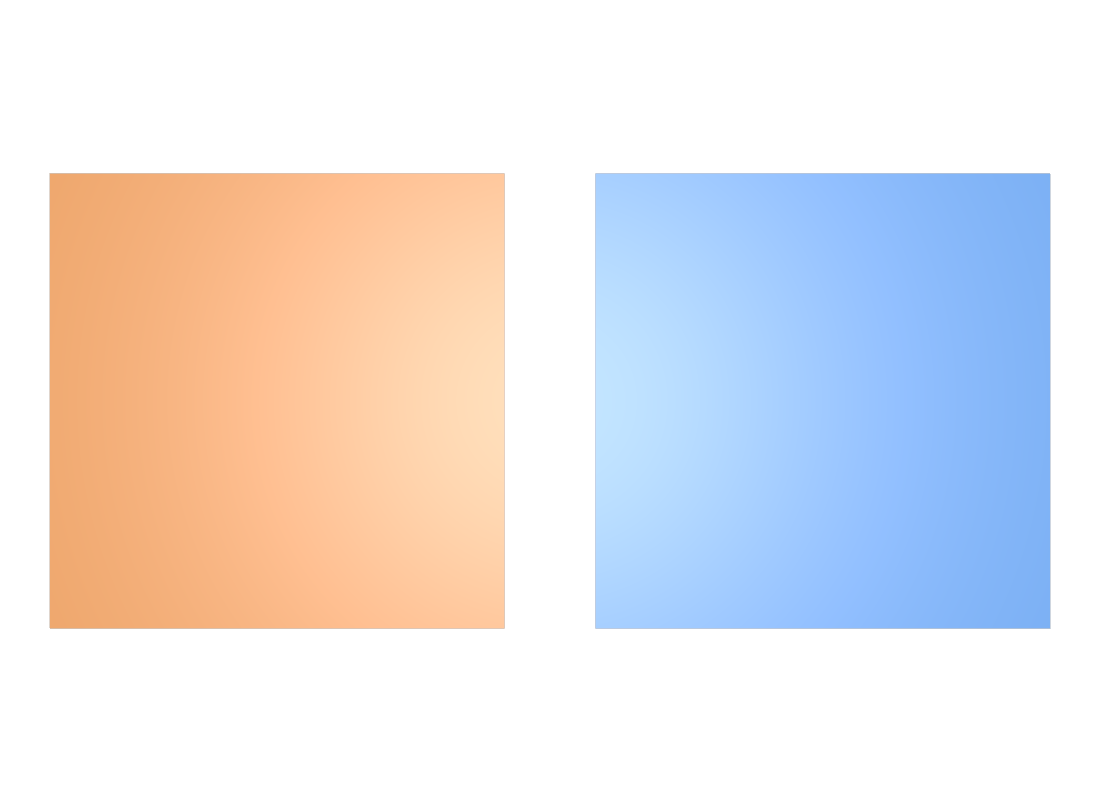
\includegraphics[width=0.88\linewidth]{figures/c17_primvar_material.png}
  \caption{The listing above rendered with \texttt{usdrecord}: both plates
  bind the \emph{same} material; the \texttt{UsdPrimvarReader} pulls each
  mesh's own \texttt{displayColor} into \texttt{diffuseColor}.}
  \label{fig:primvar-material}
\end{figure}

\begin{figure}[ht]
  \centering
  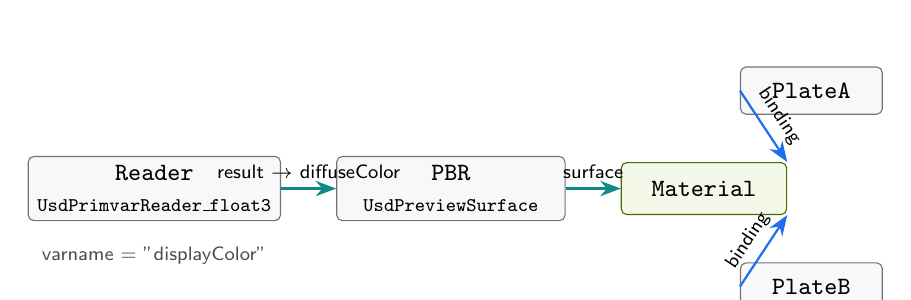
\begin{tikzpicture}[node distance=4mm and 7mm]
    \node[primbox, minimum width=2.9cm, align=center] (reader) {Reader\\ \scriptsize UsdPrimvarReader\_float3};
    \node[primbox, minimum width=2.9cm, align=center, right=of reader] (pbr) {PBR\\ \scriptsize UsdPreviewSurface};
    \node[layerbox, minimum width=2.1cm, right=of pbr] (mat) {Material};
    \node[primbox, minimum width=1.8cm, above right=6mm and -6mm of mat] (ma) {PlateA};
    \node[primbox, minimum width=1.8cm, below right=6mm and -6mm of mat] (mb) {PlateB};
    \draw[varArc] (reader) -- node[arcLabel] {result $\to$ diffuseColor} (pbr);
    \draw[varArc] (pbr) -- node[arcLabel] {surface} (mat);
    \draw[refArc] (ma.west) -- node[arcLabel] {binding} (mat.north east);
    \draw[refArc] (mb.west) -- node[arcLabel] {binding} (mat.south east);
    \node[notetext, below=2mm of reader] {varname = "displayColor"};
  \end{tikzpicture}
  \caption{The same network as a graph: connections flow left to right;
  bindings are relationships from gprims to the material.}
  \label{fig:shade-graph}
\end{figure}

\begin{ExamTip}
Why this pattern is the exam favorite: it scales. One shared material +
per-prim primvars keeps instancing intact (Content Aggregation chapter) and
avoids a material explosion --- exactly the reasoning Sample Question 10
rewards.
\end{ExamTip}

\subsection{Walking a network in code}\label{sec:vis-walk}\objref{8.2, 8.3}
Everything is prims and properties, so the network is introspectable ---
this is also how validators check shading:

\begin{lstlisting}[language=Python]
from pxr import Usd, UsdShade

stage = Usd.Stage.Open("shaded.usda")
mesh = stage.GetPrimAtPath("/Scene/PlateA")

material, rel = UsdShade.MaterialBindingAPI(mesh).ComputeBoundMaterial()
print(material.GetPath())               # /Scene/Looks/Painted

src = material.GetSurfaceOutput().GetConnectedSource()
pbr = UsdShade.Shader(src[0].GetPrim())
print(pbr.GetIdAttr().Get())            # UsdPreviewSurface

rsrc = pbr.GetInput("diffuseColor").GetConnectedSource()
reader = UsdShade.Shader(rsrc[0].GetPrim())
print(reader.GetIdAttr().Get(),         # UsdPrimvarReader_float3
      reader.GetInput("varname").Get()) # displayColor
\end{lstlisting}

\subsection{Textures, cameras, and a light}\label{sec:vis-tex}\objref{8.2, 8.4}
\index{UsdUVTexture}One node upgrades the network from flat color to
textured: \texttt{UsdUVTexture} reads an image, steered by a \texttt{float2}
primvar reader for UVs. The same scene carries a camera and a light ---
prims like everything else:

\begin{lstlisting}
#usda 1.0
( defaultPrim = "Scene" )
def Xform "Scene" {
    def Mesh "Plate" (
        prepend apiSchemas = ["MaterialBindingAPI"]
    )
    {
        int[] faceVertexCounts = [4]
        int[] faceVertexIndices = [0, 1, 2, 3]
        point3f[] points = [(-1, -1, 0), (1, -1, 0), (1, 1, 0), (-1, 1, 0)]
        texCoord2f[] primvars:st = [(0, 0), (1, 0), (1, 1), (0, 1)] (
            interpolation = "vertex"
        )
        rel material:binding = </Scene/Looks/Checkered>
    }
    def Scope "Looks" {
        def Material "Checkered" {
            token outputs:surface.connect = </Scene/Looks/Checkered/PBR.outputs:surface>
            def Shader "PBR" {
                uniform token info:id = "UsdPreviewSurface"
                color3f inputs:diffuseColor.connect = </Scene/Looks/Checkered/Tex.outputs:rgb>
                token outputs:surface
            }
            def Shader "Tex" {
                uniform token info:id = "UsdUVTexture"
                asset inputs:file = @./checker.png@
                float2 inputs:st.connect = </Scene/Looks/Checkered/Reader.outputs:result>
                color3f outputs:rgb
            }
            def Shader "Reader" {
                uniform token info:id = "UsdPrimvarReader_float2"
                string inputs:varname = "st"
                float2 outputs:result
            }
        }
    }
    def Camera "Cam" {
        float focalLength = 35
        float2 clippingRange = (0.1, 1000)
        double3 xformOp:translate = (0, 0, 6)
        uniform token[] xformOpOrder = ["xformOp:translate"]
    }
    def DistantLight "Sun" {
        float inputs:intensity = 1000
    }
}
\end{lstlisting}

\begin{figure}[ht]
  \centering
  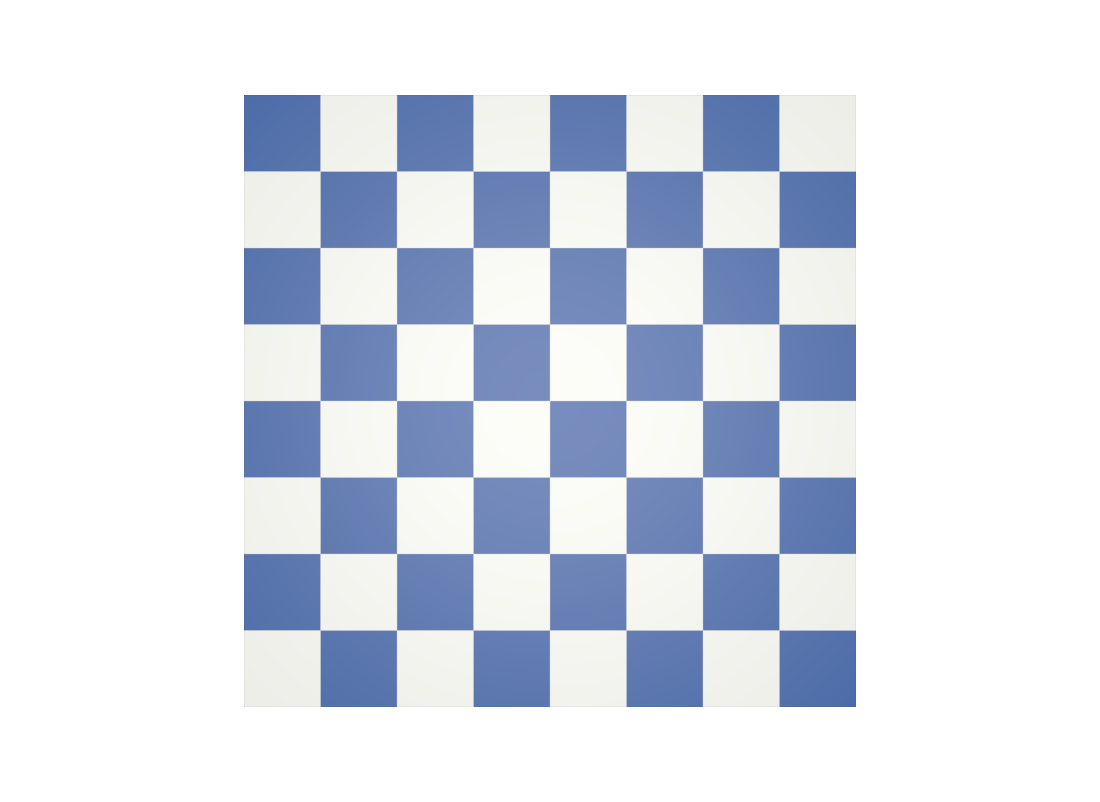
\includegraphics[width=0.8\linewidth]{figures/c17_textured.png}
  \caption{The listing rendered with \texttt{usdrecord --camera /Scene/Cam}:
  \texttt{UsdUVTexture} drives \texttt{diffuseColor}, the authored
  \texttt{DistantLight} does the lighting, the authored \texttt{Camera}
  frames the shot --- the whole render pipeline as scene description.}
  \label{fig:textured}
\end{figure}

\noindent The chain to memorize: \texttt{primvars:st} $\to$
\texttt{UsdPrimvarReader\_float2} $\to$ \texttt{UsdUVTexture.st}; the
texture's \texttt{rgb} output $\to$ \texttt{diffuseColor}. Cameras
(\texttt{UsdGeomCamera}: \texttt{focalLength}, \texttt{clippingRange},
projection) and lights complete the picture: a renderer needs nothing that
is not on the stage.\index{camera}

\subsection{Per-face materials: GeomSubset}\label{sec:vis-subset}\objref{8.3}
\index{GeomSubset}Different materials on different faces of \emph{one} mesh
--- no splitting:

\begin{lstlisting}
#usda 1.0
( defaultPrim = "Plate" )
def Mesh "Plate" (
    prepend apiSchemas = ["MaterialBindingAPI"]
)
{
    int[] faceVertexCounts = [4, 4]
    int[] faceVertexIndices = [0, 1, 2, 3, 2, 3, 4, 5]
    point3f[] points = [(-1, 0, -1), (1, 0, -1), (1, 0, 1), (-1, 0, 1),
        (1, 0, 3), (-1, 0, 3)]
    def GeomSubset "Front" {
        uniform token elementType = "face"
        int[] indices = [0]
        uniform token familyName = "materialBind"
    }
}
\end{lstlisting}

\noindent A subset names faces by index; \texttt{familyName =
"materialBind"} marks it as a binding target --- author
\texttt{material:binding} on the \emph{subset} prim exactly as on a mesh.
Subsets in a binding family should partition the faces: every face in
exactly one subset.

\begin{Gotcha}
GeomSubset relies entirely on \emph{face indices} --- change the topology
(triangulate, delete faces, re-export from a DCC) and every subset silently
points at different faces. Validate subsets after any topology-touching
step; this is a favorite ``unexpected visual result'' on round-trips.
\end{Gotcha}

\subsection{Purpose and visibility}\label{sec:vis-purpose}\objref{5.5, 6.4}
\index{purpose}\index{visibility}Two imageable controls decide what draws:

\begin{lstlisting}
#usda 1.0
( defaultPrim = "Rig" )
def Xform "Rig" {
    token visibility = "invisible"
    def Sphere "ProxySphere" {
        uniform token purpose = "proxy"
    }
    def Sphere "RenderSphere" {
        uniform token purpose = "render"
    }
}
\end{lstlisting}

\begin{lstlisting}[language=Python]
from pxr import Usd, UsdGeom

stage = Usd.Stage.Open("purpose.usda")
proxy = UsdGeom.Imageable(stage.GetPrimAtPath("/Rig/ProxySphere"))
print(proxy.ComputeVisibility())   # invisible -- inherited from /Rig
print(proxy.ComputePurpose())      # proxy
\end{lstlisting}

\noindent\texttt{visibility} (\texttt{inherited}/\texttt{invisible}) flows
down namespace --- an invisible ancestor hides the subtree.
\texttt{purpose} tags subtrees for consumers: viewports draw
\texttt{proxy}, final renders draw \texttt{render}, \texttt{guide} is for
rig helpers, and \texttt{default} draws everywhere.

\subsection{Lights are prims: UsdLux}
\index{UsdLux}Lighting follows the same schema logic as geometry and
shading. Common controls (\texttt{inputs:intensity}, \texttt{inputs:color},
\texttt{inputs:exposure}) come from \texttt{LightAPI}; light types add their
own (\texttt{DistantLight} has \texttt{inputs:angle} --- the sun's angular
size); \texttt{ShadowAPI} and \texttt{ShapingAPI} layer on shadow tinting
and IES-style shaping:

\begin{lstlisting}
#usda 1.0
( defaultPrim = "Sun" )
def DistantLight "Sun" {
    float inputs:intensity = 500
    float inputs:angle = 0.53
}
\end{lstlisting}

\begin{FieldNote}
For this domain, \texttt{usdview} is all the practice tooling you need ---
no Omniverse, no special hardware. Every render in this book was produced
with stock \texttt{usdrecord} and \texttt{usdview} on the scenes printed
beside it.
\end{FieldNote}

\DrillsTitle
\subsection*{Drill 1: Material binding}
Write a minimal example that binds a material at \texttt{/World/Looks/MyMat}
to \texttt{/World/Geo/MyMesh}.
\AnswerLines{10}
\begin{DrillSolution}
On the mesh prim: apply the schema and author the relationship ---
\texttt{prepend apiSchemas = ["MaterialBindingAPI"]} in the prim metadata,
and \texttt{rel material:binding = </World/Looks/MyMat>} in the body. In
Python: \texttt{UsdShade.MaterialBindingAPI.Apply(prim).Bind(material)}.
Verify with \texttt{ComputeBoundMaterial()} --- binding resolution respects
strength and ancestors, so trust the computed answer, not your eyes.
\end{DrillSolution}

\subsection*{Drill 2: GeomSubset use-case}
Describe when you would use GeomSubset and what data it relies on.
\AnswerLines{6}
\begin{DrillSolution}
Multiple materials on one mesh (label vs glass of a bottle) without
splitting geometry. It relies on \texttt{elementType = "face"} plus face
\emph{indices}, grouped under \texttt{familyName = "materialBind"} --- which
is why topology changes invalidate subsets.
\end{DrillSolution}

\subsection*{Drill 3: Network reading}
Without running it, predict the three printed lines of the
``walking a network'' listing, then run it mentally backwards: which edit
would make both plates render gray?
\AnswerLines{6}
\begin{DrillSolution}
It prints the material path, \texttt{UsdPreviewSurface}, and
\texttt{UsdPrimvarReader\_float3 displayColor}. Gray plates: break the chain
--- e.g.\ \texttt{varname} naming a primvar the meshes don't have (the
reader returns its fallback), or disconnecting
\texttt{inputs:diffuseColor}.
\end{DrillSolution}

\section*{Checkpoint Questions}
\addcontentsline{toc}{section}{Checkpoint Questions}

\noindent\textbf{CQ1.} One mesh must show different colors in viewport
preview vs final render. Sketch the cheapest USD-native setup.
\begin{DrillSolution}
Two sibling subtrees under the asset: a \texttt{purpose = "proxy"} version
(cheap shading) and a \texttt{purpose = "render"} version --- the renderer's
purpose selection switches; no variant or material surgery needed.
\end{DrillSolution}

\noindent\textbf{CQ2.} \texttt{ComputeBoundMaterial()} returns nothing for a
mesh that clearly has \texttt{material:binding} authored. Two likely causes?
\begin{DrillSolution}
The binding targets a prim that doesn't compose (outside
\texttt{defaultPrim} when referenced --- Sample Question 12), or the
\texttt{MaterialBindingAPI} schema isn't applied so the binding is ignored
by schema-strict consumers. Check the target's existence first.
\end{DrillSolution}

\noindent\textbf{CQ3.} Which API holds \texttt{inputs:intensity} shared by
every light type, and which API would you add for light-cone shaping?
\begin{DrillSolution}
\texttt{LightAPI} carries the shared inputs (intensity, color, exposure);
\texttt{ShapingAPI} adds cone/focus/IES controls. (\texttt{ShadowAPI} is the
third of the family --- shadow enable/color/falloff.)
\end{DrillSolution}

\subsection*{Mini-checklist (tick when mastered)}
\begin{itemize}[leftmargin=*]
  \item[$\square$] I can author the primvar-reader network from memory.
  \item[$\square$] I can walk mesh $\to$ material $\to$ shaders in Python.
  \item[$\square$] I know why GeomSubsets break on topology changes.
  \item[$\square$] I can place purpose/visibility on the right prim the first time.
\end{itemize}


\part{Practice}
\input{chapters/20-sample-questions}
\clearpage
\section*{Answer Key}
\addcontentsline{toc}{section}{Answer Key}
\label{sec:sample-key}

Every composition scenario in this key was verified by composing the actual
layers with OpenUSD and inspecting the result --- not by reasoning alone.

\Question{1 --- A}
\texttt{defaultPrim}\index{defaultPrim} is layer metadata naming the prim that
consumers compose when they reference or payload the layer \emph{without}
specifying a prim path. It has nothing to do with materials, timeCodes, or
schema definitions.

\Question{2 --- C: (0, 1, 0)}
LIVRPS\index{LIVRPS}: the \emph{Local} opinion in \texttt{scene.usda} is
stronger than anything brought in by the two \emph{References}, so $(0,1,0)$
wins. Between the references themselves, the earlier list entry
(\texttt{chair\_base.usda}) would beat the later one --- relevant only for
opinions the stronger layers do not author.
Figure~\ref{fig:key-q2} makes it visible: a proxy sphere parented under
\texttt{/World/Chair} picks up the composed transform, while gray markers sit
at the four candidate positions.

\begin{figure}[ht]
  \centering
  \begin{tikzpicture}
    \node[anchor=south west, inner sep=0] (img)
      {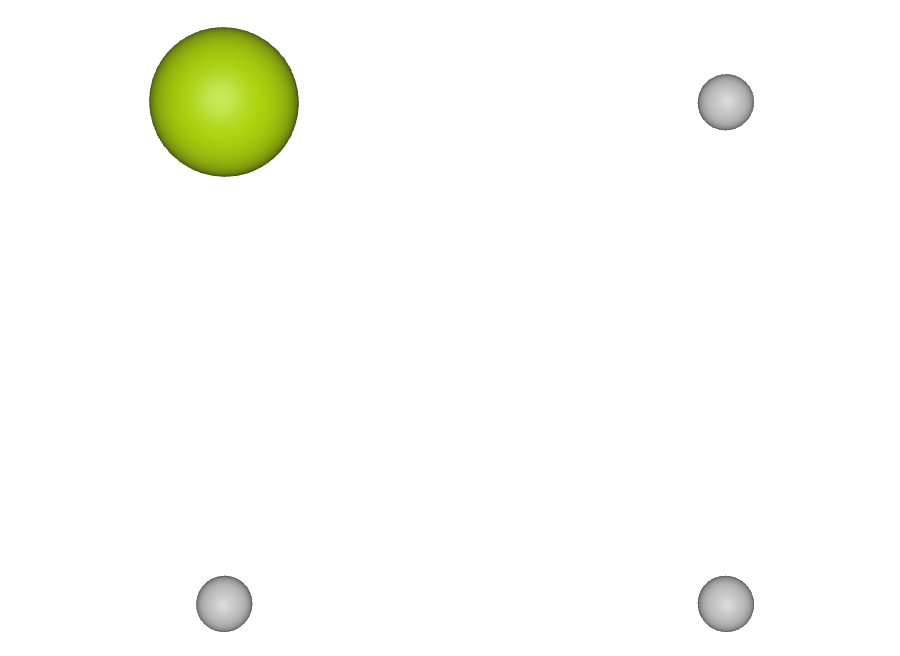
\includegraphics[width=0.62\linewidth]{figures/q02_chair_options.png}};
    \begin{scope}[x={(img.south east)}, y={(img.north west)}]
      \node[notetext] at (0.245,0.185) {A $(0,0,0)$};
      \node[notetext] at (0.80,0.185)  {B $(1,0,0)$};
      \node[notetext] at (0.80,0.72)   {D $(1,1,0)$};
      \node[notetext, draw=usdgreen!60!black, fill=white, rounded corners=1pt]
        (c) at (0.47,0.60) {C $(0,1,0)$ --- composed result};
      \draw[subArc] (c.north west) -- (0.295,0.78);
    \end{scope}
  \end{tikzpicture}
  \caption{Question 2, rendered with \texttt{usdrecord}: gray markers sit at
  the four answer options; the sphere under \texttt{/World/Chair} composes to
  C.}
  \label{fig:key-q2}
\end{figure}

\Question{3 --- A, B, D}
Topology lives in three attributes: \texttt{points},
\texttt{faceVertexCounts}, and \texttt{faceVertexIndices} --- counts say how
many vertices each face consumes, indices say which ones. \texttt{normals}
can be computed (or come from subdivision), and
\texttt{primvars:\allowbreak displayColor} is cosmetic --- both optional.

\Question{4 --- C: 1,500}
Each of the 500 triangular faces consumes three indices:
$500 \times 3 = 1{,}500$ entries. \texttt{faceVertexCounts} would hold 500
entries, each equal to 3.

\Question{5 --- A, B}
Move points $\Rightarrow$ recompute \texttt{extent}\index{extent} (bounds are
authored, not derived on the fly). Change topology $\Rightarrow$ keep
\texttt{faceVertexCounts} consistent with \texttt{faceVertexIndices}. The
pairs in C and D are independent properties, not synchronization invariants.

\Question{6 --- C}
Adding properties to \emph{existing} prim types is what applied API
schemas\index{API schema} do, and those derive from
\texttt{UsdAPISchemaBase}. \texttt{UsdTyped} is the base for IsA (typed)
schemas that define new prim types; \texttt{UsdSchemaBase} is the common
ancestor you do not subclass directly; \texttt{UsdPhysicsBase} does not exist.

\Question{7 --- B, C}
Composition's headline wins are collaboration (people own separate layers of
the same stage without write conflicts) and nondestructive overrides (stronger
opinions on top, original data intact). A confuses USD with version control
--- any file format can live in git. D inverts reality: more layers add
composition cost; they do not optimize access.

\Question{8 --- A, B}
Naming/structure conventions and validation at boundaries are what keep a
pipeline alive as it grows. C is the trap answer: asset structures evolve, so
design for change rather than pretending to finalize one up front. D is dogma
--- production pipelines exchange with DCC-native formats all the time.

\Question{9 --- B}
The \texttt{UsdGeomImageable}\index{UsdGeomImageable} schema carries what
every \emph{renderable} prim needs: \texttt{visibility}, \texttt{purpose},
and primvar plumbing. Concrete geometric properties live further down the
hierarchy (\texttt{Boundable}, \texttt{Gprim}); material assignment belongs to
\texttt{UsdShade} (\texttt{MaterialBindingAPI}).

\Question{10 --- B}
Expose the parameters you expect to vary as inputs on the material's public
interface; consumers then override them per use, instead of forking a material
per combination (C) or hardcoding values (A).

\Question{11 --- B}
\texttt{metersPerUnit}\index{metersPerUnit} is descriptive metadata; USD
performs \emph{no} automatic unit conversion when referencing. Meter-unit
geometry (1.0) interpreted inside a centimeter-unit stage (0.01) reads
100$\times$ too small. Correcting it is the referencing pipeline's job ---
typically a corrective scale on the referencing prim.

\Question{12 --- C}
The export parses cleanly --- verified --- but \texttt{defaultPrim} is
\texttt{World}, and the binding targets \texttt{/Materials/metal}, which lives
\emph{outside} that hierarchy. Reference this layer into another stage and
\texttt{/Materials} never composes; the binding dangles.
\texttt{bindMaterialAs} metadata (A) is legal on a binding relationship;
geom subsets (B) are optional, not required; D inverts the binding model.

\Question{13 --- B}
Composed and verified: the stage \emph{does} resolve
\texttt{loftedColor = blue}, yet the cube stays red. The artist's local
\texttt{over} on \texttt{Cube} in \texttt{main.usda} authors a direct
\texttt{color = red} selection, and a Local opinion beats the selection
authored inside the \texttt{loftedColor} variant (V in LIVRPS). A is backwards
--- the selection in \texttt{contents.usda} is the \emph{weakest} of the
three. C misreads the mechanism: the blue variant does select
\texttt{color = blue}; it simply loses. D is false --- variant selections can
be authored on any prim spec, including in \texttt{main.usda}.
Figure~\ref{fig:key-q13} is the composed stage, rendered.

\begin{figure}[ht]
  \centering
  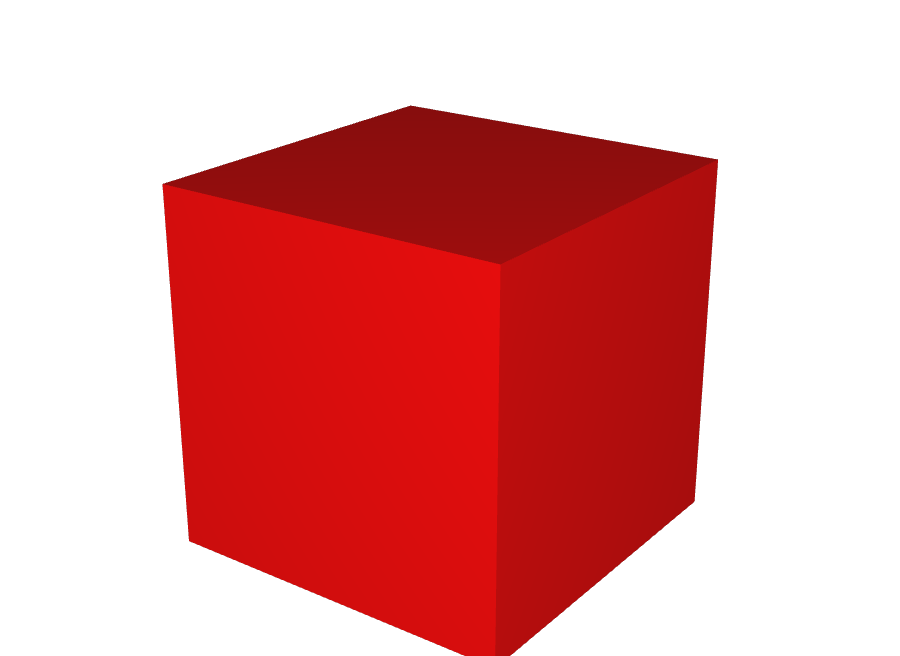
\includegraphics[width=0.42\linewidth]{figures/q13_cube_red.png}
  \caption{Question 13 rendered with \texttt{usdrecord}: the composed stage
  draws a red cube, exactly as answer B predicts.}
  \label{fig:key-q13}
\end{figure}

\chapter{Study-Guide Coverage Map}
\setlength{\tabcolsep}{5pt}

Every numbered objective of NVIDIA's \emph{NCP: OpenUSD Development Exam
Study Guide} (v1.1.0), and where this book covers it --- the section numbers
are clickable. The same objective numbers appear as margin tags next to the
covering passages. Objectives the guide repeats across domains point at the
same sections on purpose.

\section*{1 --- Composition (23\%)}
\begin{tabular}{@{}p{0.45in}p{2.40in}p{1.55in}@{}}
1.1 & Change the strength of an opinion & \S\ref{sec:c-stacks}, \S\ref{sec:c-livrps} \\
1.2 & Instancing style for different scales & \S\ref{sec:ca-sg}, \S\ref{sec:ca-pi} \\
1.3 & References vs payloads vs sublayers & \S\ref{sec:c-refs}--\ref{sec:c-payloads}, \S\ref{sec:pd-subref} \\
1.4 & Same animation, different time-offsets & \S\ref{sec:c-offsets} \\
1.5 & Layering for multi-user workflows & \S\ref{sec:c-stacks}, \S\ref{sec:pd-subref} \\
1.6 & Explain LIVERPS & \S\ref{sec:c-livrps} \\
1.7 & When variants are (not) appropriate & \S\ref{sec:c-variants} \\
1.8 & Why opinions do not take effect & \S\ref{sec:c-livrps}, \S\ref{sec:dbg-repro}--\ref{sec:dbg-mute} \\
1.9 & Prepare assets for external delivery & \S\ref{sec:c-edit}, \S\ref{sec:pd-deliver} \\
1.10 & Remove properties from instanced prims & \S\ref{sec:ca-edit} \\
1.11 & Split a monolithic asset & \S\ref{sec:c-edit}, \S\ref{sec:pd-iface} \\
\end{tabular}

\section*{2 --- Content Aggregation (10\%)}
\begin{tabular}{@{}p{0.45in}p{2.40in}p{1.55in}@{}}
2.1 & Add a PointInstancer prototype & \S\ref{sec:ca-pi} \\
2.2 & Edit an instanceProxy without breaking & \S\ref{sec:ca-edit} \\
2.3 & Hide PointInstancer instances & \S\ref{sec:ca-pi} \\
2.4 & Manage instances for reuse at scale & \S\ref{sec:ca-sg} \\
2.5 & Remove properties from instanced prims & \S\ref{sec:ca-edit} \\
\end{tabular}

\section*{3 --- Customizing USD (6\%)}
\begin{tabular}{@{}p{0.45in}p{2.40in}p{1.55in}@{}}
3.1 & Build a plug-in against a USD version & \S\ref{sec:cu-map}, \S\ref{sec:cu-build} \\
3.2 & Build USD from source, custom deps & \S\ref{sec:cu-build} \\
3.3 & Create custom model kinds & \S\ref{sec:cu-kinds}, \S\ref{sec:pd-kinds} \\
3.4 & Create custom schemas & \S\ref{sec:cu-schemas}--\ref{sec:cu-api} \\
3.5 & Integrate a custom resolver & \S\ref{sec:cu-ext}, \S\ref{sec:pd-res} \\
3.6 & Schemas for nonstandard data & \S\ref{sec:cu-schemas}, \S\ref{sec:de-nonstd} \\
3.7 & SceneIndex plug-in for Hydra prims & \S\ref{sec:cu-ext} \\
3.8 & In-memory renderable primitives & \S\ref{sec:cu-ext} \\
\end{tabular}

\section*{4 --- Data Exchange (15\%)}
\begin{tabular}{@{}p{0.45in}p{2.40in}p{1.55in}@{}}
4.1 & Convert to common formats, fidelity & \S\ref{sec:de-map} \\
4.2 & Conceptual data mapping documents & \S\ref{sec:de-map} \\
4.3 & USDC vs USDA trade-offs & \S\ref{sec:de-enc} \\
4.4 & Round-trip pipeline in a DCC & \S\ref{sec:de-rt} \\
4.5 & Nonstandard attrs during import/export & \S\ref{sec:de-nonstd} \\
4.6 & Validator for exported assets & \S\ref{sec:de-clean}, \S\ref{sec:de-val} \\
4.7 & Write an exporter/converter & \S\ref{sec:de-trav} \\
4.8 & Write or extend an importer & \S\ref{sec:de-rt} \\
\end{tabular}

\section*{5 --- Data Modeling (13\%)}
\begin{tabular}{@{}p{0.45in}p{2.40in}p{1.55in}@{}}
5.1 & Add a primvar to a mesh & \S\ref{sec:dm-primvars}--\ref{sec:dm-api} \\
5.2 & Choose appropriate value types & \S\ref{sec:dm-types} \\
5.3 & Represent custom metadata & \S\ref{sec:dm-api} \\
5.4 & Retrieve properties of a prim & \S\ref{sec:dm-tax}, \S\ref{sec:dm-api} \\
5.5 & Causes of unexpected visual results & \S\ref{sec:dm-primvars}, \S\ref{sec:vis-purpose} \\
5.6 & Update extent after updating points & \S\ref{sec:dm-extent} \\
\end{tabular}

\section*{6 --- Debugging and Troubleshooting (11\%)}
\begin{tabular}{@{}p{0.45in}p{2.25in}p{1.70in}@{}}
6.1 & When SdfChangeBlock helps & \S\ref{sec:dbg-perf} \\
6.2 & Why opinions do not take effect & \S\ref{sec:dbg-repro}--\ref{sec:dbg-mute} \\
6.3 & Asset-management issues & \S\ref{sec:dbg-mute}, \S\ref{sec:c-refs}, \S\ref{sec:pd-paths} \\
6.4 & Causes of unexpected visual results & \S\ref{sec:dm-primvars}, \S\ref{sec:vis-purpose} \\
6.5 & Diagnostics and profiling facilities & \S\ref{sec:dbg-diag} \\
\end{tabular}

\section*{7 --- Pipeline Development (14\%)}
\begin{tabular}{@{}p{0.45in}p{2.40in}p{1.55in}@{}}
7.1 & Convert to common formats & \S\ref{sec:de-map}, \S\ref{sec:pd-deliver} \\
7.2 & Document asset structure guidelines & \S\ref{sec:pd-iface}--\ref{sec:pd-kinds} \\
7.3 & USDC vs USDA trade-offs & \S\ref{sec:de-enc} \\
7.4 & Round-trip pipelines & \S\ref{sec:de-rt} \\
7.5 & Custom resolvers for asset paths & \S\ref{sec:pd-res} \\
7.6 & Represent custom metadata & \S\ref{sec:pd-iface}, \S\ref{sec:dm-api} \\
7.7 & Validate asset path formatting & \S\ref{sec:pd-paths} \\
7.8 & Write or extend an importer & \S\ref{sec:de-rt} \\
\end{tabular}

\section*{8 --- Visualization (8\%)}
\begin{tabular}{@{}p{0.45in}p{2.25in}p{1.70in}@{}}
8.1 & Add a primvar to a mesh & \S\ref{sec:dm-primvars} \\
8.2 & Assign UsdPreviewSurface materials & \S\ref{sec:vis-net}--\ref{sec:vis-walk} \\
8.3 & Bind materials to a mesh & \S\ref{sec:vis-walk}--\ref{sec:vis-subset} \\
8.4 & PreviewSurface network from a primvar & \S\ref{sec:vis-net} \\
\end{tabular}


\backmatter
\addcontentsline{toc}{chapter}{Index}
\printindex
\end{document}
